\documentclass[UTF8,zihao=-4,openany,fontset=none]{ctexrep}

\usepackage[a4paper,top=2.75cm,bottom=2.55cm,left=2.75cm,right=2.55cm,headsep=0.65cm]{geometry}
\usepackage{graphicx}
\usepackage{booktabs}
\usepackage{amsmath}
\usepackage{longtable}
\usepackage{tabularx}
\usepackage{array}
\usepackage[table]{xcolor}
\usepackage{hyperref}
\usepackage{caption}
\usepackage{float}
\usepackage{etoolbox}
\usepackage{listings}
\usepackage{fancyhdr}
\usepackage{tikz}
\usetikzlibrary{arrows.meta,positioning}

\graphicspath{{figures/}}
\setmainfont{Times New Roman}
\setsansfont{Times New Roman}
\setCJKmainfont[AutoFakeBold=2.5]{Songti SC}
\setCJKsansfont[AutoFakeBold=2.5]{Songti SC}
\setCJKmonofont[AutoFakeBold=2.0]{Songti SC}

\definecolor{bfPrimary}{HTML}{202020}
\definecolor{bfInk}{HTML}{202020}
\definecolor{bfMuted}{HTML}{666666}
\definecolor{bfRule}{HTML}{D6D6D6}
\definecolor{bfPanel}{HTML}{F6F6F6}
\definecolor{bfCode}{HTML}{F7F7F7}

\hypersetup{
  colorlinks=true,
  linkcolor=black,
  citecolor=black,
  urlcolor=black,
  pdfauthor={Boring Financial Team},
  pdftitle={Boring Financial 智能账单分类系统项目报告}
}

\linespread{1.18}
\setlength{\parskip}{0.2em}
\setlength{\tabcolsep}{7pt}
\renewcommand{\arraystretch}{1.32}
\arrayrulecolor{bfRule}
\urlstyle{same}
\sloppy

\ctexset{
  chapter = {
    format = \raggedright\bfseries\zihao{2}\color{bfInk},
    nameformat = \bfseries\zihao{4}\color{bfMuted},
    numberformat = \bfseries\zihao{4}\color{bfMuted},
    titleformat = \bfseries\zihao{2}\color{bfInk},
    aftername = \quad,
    beforeskip = 0.1em,
    afterskip = 1.45em
  },
  section = {
    format = \raggedright\bfseries\zihao{3}\color{bfInk},
    beforeskip = 1.25em,
    afterskip = 0.65em
  },
  subsection = {
    format = \raggedright\bfseries\zihao{4}\color{bfInk},
    beforeskip = 1em,
    afterskip = 0.45em
  }
}

\newcommand{\headingneedspace}[1]{%
  \par
  \begingroup
    \dimen0=\pagegoal
    \advance\dimen0 by -\pagetotal
    \dimen2=#1\baselineskip
    \ifdim\dimen0<\dimen2
      \newpage
    \fi
  \endgroup
}
\pretocmd{\section}{\headingneedspace{10}}{}{}
\pretocmd{\subsection}{\headingneedspace{7}}{}{}

\captionsetup{
  font=small,
  labelfont={bf,color=bfInk},
  textfont={color=bfInk},
  labelsep=quad,
  skip=8pt
}

\pagestyle{fancy}
\fancyhf{}
\fancyhead[L]{\small\color{bfMuted}\projectname}
\fancyhead[R]{\small\color{bfMuted}\leftmark}
\fancyfoot[C]{\small\color{bfMuted}\thepage}
\renewcommand{\headrulewidth}{0.4pt}
\renewcommand{\footrulewidth}{0pt}
\renewcommand{\headrule}{\hbox to\headwidth{\color{bfRule}\leaders\hrule height \headrulewidth\hfill}}
\setlength{\headheight}{24pt}

\fancypagestyle{plain}{
  \fancyhf{}
  \fancyfoot[C]{\small\color{bfMuted}\thepage}
  \renewcommand{\headrulewidth}{0pt}
}

\lstset{
  basicstyle=\ttfamily\small,
  breaklines=true,
  columns=fullflexible,
  frame=single,
  framesep=6pt,
  framerule=0.4pt,
  rulecolor=\color{bfRule},
  backgroundcolor=\color{bfCode}
}

\newcommand{\projectname}{Boring Financial 智能账单分类系统}
\newcommand{\uiscreenshot}[1]{%
  \includegraphics[
    width=0.88\textwidth,
    height=0.24\textheight,
    keepaspectratio
  ]{#1}%
}
\newcommand{\placeholderfigure}[2]{%
  \begin{figure}[H]
    \centering
    \fcolorbox{bfRule}{bfPanel}{%
      \begin{minipage}[c][4.2cm][c]{0.84\textwidth}
        \centering\color{bfMuted}#1
      \end{minipage}%
    }
    \caption{#2}
  \end{figure}
}

\tikzset{
  umlclass/.style={
    draw=bfRule,
    fill=bfPanel,
    rounded corners=1pt,
    align=left,
    text width=3.7cm,
    inner sep=4pt,
    font=\ttfamily\scriptsize
  },
  umlrel/.style={-{Latex[length=2mm]}, draw=bfMuted, line width=0.45pt},
  umlinherit/.style={-{Triangle[length=2mm,width=2mm]}, draw=bfMuted, line width=0.45pt}
}

\newcommand{\classbox}[4][]{%
  \node[umlclass,#1] (#2) {%
    \textbf{#3}\\[-0.2em]
    \rule{\linewidth}{0.2pt}\\[-0.15em]
    #4%
  };
}

\begin{document}

\newgeometry{top=2.1cm,bottom=2.1cm,left=2.35cm,right=2.35cm}
\begin{titlepage}
  \thispagestyle{empty}
  \centering
  \vspace*{3.2cm}
  {\zihao{1}\bfseries \projectname\par}
  \vspace{2.2cm}
  {\zihao{4}
  \begin{tabular}{rl}
    项目成员：& 郑博文、林子尧、单彬、沈柔希 \\
    \addlinespace[0.45cm]
    项目周期：& 2026 年 3 月 -- 2026 年 6 月
  \end{tabular}
  }
\end{titlepage}
\restoregeometry

\pagenumbering{Roman}
\tableofcontents
\clearpage

\pagenumbering{arabic}

\chapter{项目概述}

\section{项目背景与问题分析}

在个人财务管理场景中，自动记账工具（如微信账单导出、支付宝账单导出）已成为日常财务整理的重要手段。然而，传统记账软件在自动分类环节存在显著短板，直接影响统计分析的准确性。一个典型且普遍的场景是：当用户向校园一卡通充值时，账单上的商户名称可能仅显示为「东南大学」。基于关键词匹配的传统分类引擎很容易将其归入「学习」类别，但从真实消费意图来看，这笔交易更接近于「餐饮/校园卡充值」。这种语义误判一旦发生，不仅会扭曲用户的消费结构认知，还会在没有校正机制的情况下持续污染后续的财务统计。

进一步分析，个人用户在整理微信、支付宝账单时通常会遇到三类共性问题：

\begin{enumerate}
  \item \textbf{自动分类依赖浅层规则}：传统分类引擎仅根据商户名或关键词做简单匹配，难以理解「在便利店买口罩」和「在便利店买零食」之间的消费意图差异。
  \item \textbf{分类依据不透明}：用户不知道一笔交易为什么被归入某个类别，缺乏解释性，因而无法判断分类是否可信。
  \item \textbf{误判缺少校正入口}：当分类出错时，用户要么被动接受错误结果，要么需要逐个手动修改，缺乏一个高效、可控的人工校正机制。
\end{enumerate}

Boring Financial 正是针对上述问题设计的解决方案。系统围绕“导入—大模型语义初分—人工校正—多维度分析—报表输出”的完整业务流程展开，将原始账单转换为语义准确、可解释、可修正的财务分析结果，同时引入消费人格画像和家庭组织聚合等分析维度，为用户提供比传统记账工具更深入的财务洞察。

\section{项目目标}

Boring Financial 的核心定位是一个面向个人与家庭的智能账单分类与财务分析系统。项目的具体目标如表~\ref{tab:project-goals} 所示。

\begin{table}[H]
\centering
\caption{项目目标}
\label{tab:project-goals}
\begin{tabular}{p{3.8cm}p{9.4cm}}
\toprule
\textbf{目标} & \textbf{说明} \\
\midrule
完成记账分析流程 & 支持账单导入、格式解析、大模型语义初分、人工校正、统计看板、消费人格画像、家庭组织聚合和 PDF 报表的完整流程。 \\
\addlinespace
支持多用户与数据隔离 & 用户默认只能访问自己的账单、交易、分类和报表；加入家庭组织后可按成员角色查看聚合数据，个人数据的独立性不受影响。 \\
\addlinespace
支持语义分类与人工校正 & 以大模型语义分类为主要手段，同时保留规则分类作为后备方案，并为低置信度交易提供人工校正入口，确保用户对最终分类结果拥有控制权。 \\
\addlinespace
支持工程化部署 & 提供清晰的系统架构、接口文档、开发指南、测试套件和部署说明，支持从本地开发到 Docker Compose 裸机部署的多种运行模式。 \\
\addlinespace
控制实现复杂度 & 聚焦记账分析业务流程本身，不引入支付、清算和银行级风控等超出项目范围的功能。 \\
\bottomrule
\end{tabular}
\end{table}

\section{项目范围}

\subsection{范围内功能}

\begin{table}[H]
\centering
\caption{项目范围内功能模块}
\label{tab:in-scope}
\begin{tabular}{p{3cm}p{10.2cm}}
\toprule
\textbf{模块} & \textbf{范围说明} \\
\midrule
用户认证 & 注册、登录、JSON Web Token（JWT）身份鉴别、多用户数据隔离。 \\
账单导入 & 支持微信、支付宝账单文件上传，管理导入批次状态和导入记录。 \\
账单解析 & 将不同平台的原始账单格式转换为统一的交易数据结构，支持去重。 \\
大模型初分 & 支持规则分类、缓存分类和外部大模型语义分类的组合处理流程，提供分类理由与置信度，并设置失败重试机制。 \\
人工校正 & 用户可筛选和复核低置信度交易，修正错误分类，修正结果在后续统计中体现。 \\
分类管理 & 支持系统预设分类和用户自定义分类，系统分类不可禁用。 \\
财务看板 & 展示收入、支出、结余、储蓄率、分类占比分布、Top 商户和收支趋势。 \\
消费人格 & 基于行为经济学理论生成 16 型消费人格画像、五维财务健康评分，并提供自评问卷与数据画像的偏差对比。 \\
家庭组织 & 支持创建家庭组织、管理所有者、管理员和普通成员角色，聚合家庭财务看板、家庭消费人格和家庭报表。 \\
PDF 报表 & 按日期范围和导入文件生成可下载的 PDF 财务报告。 \\
系统部署 & 支持本地开发运行、Docker Compose 多服务部署和裸机 Nginx 与 systemd 部署。 \\
\bottomrule
\end{tabular}
\end{table}

\subsection{范围外内容}

\begin{table}[H]
\centering
\caption{项目范围外内容及原因}
\label{tab:out-scope}
\begin{tabular}{p{4.2cm}p{9cm}}
\toprule
\textbf{不做内容} & \textbf{原因} \\
\midrule
支付、转账、清算 & 涉及真实资金流和金融合规要求，超出项目范围。 \\
银行级风控与审计 & 需要严格的合规流程和高安全保障，不属于记账分析业务流程的核心关注点。 \\
多机构财务管理 & 当前定位为个人与家庭的账单分类与分析工具。 \\
复杂家庭预算审批流程 & 当前家庭组织模块聚焦成员聚合和角色管理，不做多级审批流。 \\
商业化运营后台 & 系统聚焦个人使用和轻量部署，不覆盖商业运营能力。 \\
\bottomrule
\end{tabular}
\end{table}

\section{项目收益}

Boring Financial 的收益可以从多个利益相关方视角进行审视，如表~\ref{tab:benefits} 所示。

\begin{table}[H]
\centering
\caption{项目收益分析}
\label{tab:benefits}
\begin{tabular}{p{2.8cm}p{10.4cm}}
\toprule
\textbf{受益方} & \textbf{收益} \\
\midrule
普通用户 & 减少误分类带来的统计偏差，快速理解个人支出结构、消费趋势和消费行为特征。通过消费人格画像获得对自身消费心理的深层认知，通过家庭组织模块了解家庭成员的整体财务状况。 \\
\addlinespace
家庭管理员 & 可将个人账本聚合为家庭视图，了解家庭整体的收入支出情况和消费结构，无需为家庭成员创建共享账本或手动合并数据。 \\
\addlinespace
系统运维人员 & 基于清晰的模块边界、标准化的接口文档、自动化测试套件和多种部署方案，可快速搭建和维护系统运行环境。 \\
\addlinespace
项目开发团队 & 在实践中覆盖了需求分析、系统设计、编码实现、测试验证、部署运维和文档整理的全流程，积累了从单体应用到前后端分离系统的完整开发经验。 \\
\bottomrule
\end{tabular}
\end{table}

\chapter{可行性分析与规划}

\section{开发流程与选择依据}

本项目采用轻量级迭代开发流程，而非传统的瀑布模型。这一选择基于以下实际约束和工程考量：

\begin{table}[H]
\centering
\caption{开发流程选择依据}
\label{tab:process-reasons}
\begin{tabular}{p{3cm}p{10.2cm}}
\toprule
\textbf{因素} & \textbf{说明} \\
\midrule
有限的项目周期 & 项目从 3 月持续至 6 月，需要在约四个月内完成从需求分析到部署交付的全部工作，要求流程具备快速反馈和持续交付能力。 \\
\addlinespace
需求随实现迭代演化 & 不同平台的账单格式差异、大模型分类的实际效果以及前端交互体验都需要在实际实现和联调过程中不断验证和修正，难以在初始阶段完全冻结需求。 \\
\addlinespace
团队可并行推进 & 前端、后端、分类模型、测试和文档等工作可按照模块边界并行开发，迭代流程天然支持这种并行协作模式。 \\
\addlinespace
最小可行产品（MVP）优先策略 & 首先保证“导入—大模型初分—人工校正—分析—报表”的核心业务流程可运行，后续再逐步补充增强功能。 \\
\addlinespace
文档持续积累 & 各阶段的过程文档在开发过程中持续积累，在最终交付阶段统一整理为完整报告，避免期末集中赶工。 \\
\bottomrule
\end{tabular}
\end{table}

\subsection{迭代阶段与反馈机制}

系统的开发过程划分为四个阶段，阶段之间通过反馈回路进行修正：

\begin{itemize}
  \item \textbf{阶段一（3 月）：选题与需求}。确立项目目标、完成可行性研究、明确团队分工和需求范围。核心产出包括项目目标说明、可行性论证、需求列表和利益相关者分析。

  \item \textbf{阶段二（4 月）：原型与架构}。完成前端页面原型、系统架构设计、组件图、部署图，以及安全性和性能的初步设计。此阶段的架构决策为后续实现提供了稳定的技术骨架。

  \item \textbf{阶段三（5 月）：功能实现与联调}。完成核心功能的开发并进行前后端联调。实现范围覆盖用户认证、账单导入、AI 分类、人工校正、财务看板、消费人格画像、家庭组织和 PDF 报表。实现过程中发现的技术约束会反向修正架构设计，联调中发现的问题会反向修正需求定义。

  \item \textbf{阶段四（6 月）：测试、部署与报告}。完成自动化测试和手工验收测试，编写部署文档，整理最终报告和答辩材料。测试中发现的缺陷会触发对实现和设计的修正。
\end{itemize}

\begin{figure}[!htbp]
  \centering
  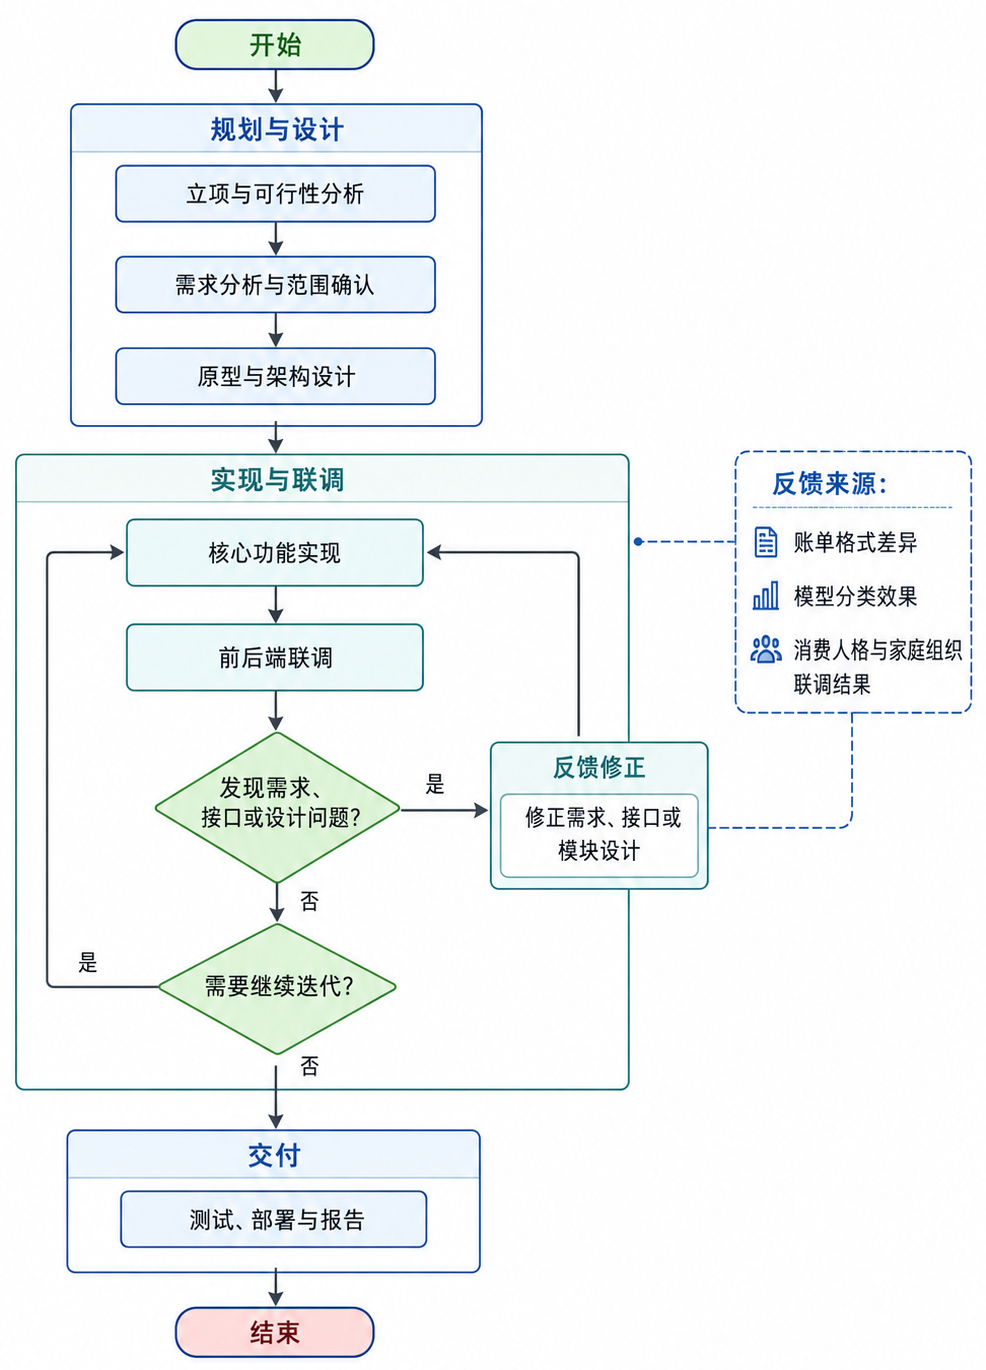
\includegraphics[
    width=0.78\textwidth,
    height=0.66\textheight,
    keepaspectratio
  ]{开发流程图.png}
  \caption{开发流程迭代图}
  \label{fig:dev-flow}
\end{figure}

\section{可行性分析}

在项目启动阶段，从五个维度对项目可行性进行了系统评估。评估结果如表~\ref{tab:feasibility} 所示。

\begin{table}[H]
\centering
\caption{多维度可行性分析}
\label{tab:feasibility}
\begin{tabular}{p{2.6cm}p{2cm}p{8.6cm}}
\toprule
\textbf{维度} & \textbf{结论} & \textbf{依据} \\
\midrule
业务可行性 & 可行 & 自动记账分类误判是真实的用户痛点，大模型语义分类结合人工校正的解决方案价值明确。消费人格画像和家庭组织聚合进一步增强了产品的差异化竞争力。 \\
\addlinespace
技术可行性 & 可行 & 技术栈选择成熟稳定：FastAPI 提供异步应用程序接口（API），Vue 3 + Element Plus 提供组件化的前端能力，SQLAlchemy 提供对象关系映射（ORM）的数据操作抽象，Docker 提供一致化的运行环境。所有技术均有丰富的社区支持和生产实践验证。 \\
\addlinespace
进度可行性 & 可行 & 四个月的项目周期可以支撑四阶段的迭代开发节奏。四人团队按前端、后端、模型与测试的模块边界并行推进，核心业务流程可以在两个月内形成最小可行版本。 \\
\addlinespace
资源可行性 & 可行 & 开发设备使用团队成员的本地电脑，无需额外硬件投入。Git、Docker、PostgreSQL、Redis 等工具均采用开源或免费方案。模型服务支持本地模拟和规则后备方案，可灵活控制对商用 API 的依赖。 \\
\addlinespace
经济可行性 & 可行 & 项目预算较低，主要成本为成员的开发时间和可选的大模型 API 调用费用（可通过规则后备方案和本地模型服务进一步控制）。 \\
\addlinespace
维护可行性 & 基本可行 & 采用统一代码仓库、分层后端架构和前端组件化设计，配合接口文档和自动化测试，为后续维护提供了可追溯的技术基础。 \\
\bottomrule
\end{tabular}
\end{table}

\subsection{方案选型分析}

在系统核心分类策略上，项目初期评估了三种备选方案，如表~\ref{tab:alternatives} 所示。

\begin{table}[H]
\centering
\small
\caption{分类策略方案对比}
\label{tab:alternatives}
\begin{tabularx}{0.98\textwidth}{p{2.1cm} X X X}
\toprule
\textbf{评价维度} & \textbf{仅关键词规则} & \textbf{仅大模型自动分类} & \textbf{大模型初分 + 人工校正} \\
\midrule
语义准确性 & 对固定商户和关键词稳定，但难以识别真实消费意图 & 语义理解能力较强，但仍可能产生不可预测误判 & 自动建议结合人工最终确认，降低关键误判对统计的长期影响 \\
\hline
响应与可靠性 & 本地执行快，不依赖外部服务 & 受网络、配额和模型服务可用性影响 & 缓存与规则可快速返回；外部请求由重试池隔离并可降级 \\
\hline
成本与隐私 & 调用成本低，数据不离开本地 & 产生 API 调用成本，交易摘要可能发送至外部服务 & 通过缓存减少重复调用，并保留本地模型选项；仍需告知外部传输风险 \\
\hline
用户控制权 & 规则可解释，但普通用户难以维护完整规则集 & 用户只能接受模型结果 & 展示分类来源、置信度和理由，允许用户确定最终分类 \\
\hline
实现与维护 & 实现最简单，但规则规模增长后维护困难 & 接入简单，但异常处理和结果稳定性不足 & 实现复杂度最高，需要双分类字段、缓存、重试和校正界面 \\
\hline
结论 & 作为快速匹配与后备策略 & 不单独采用 & \textbf{作为最终方案} \\
\bottomrule
\end{tabularx}
\end{table}

最终选择“语义初分+人工校正”方案，并保留分类缓存、规则分类、本地模型和统一失败重试机制。该选择不是单纯追求模型准确率，而是在语义能力、响应时间、调用成本、隐私风险、系统可靠性和用户控制权之间取得平衡。

\section{项目计划与进度}

\subsection{工作分解结构（WBS）}

项目的核心任务分解如表~\ref{tab:wbs} 所示。各任务按模块边界划分，明确负责人、前置依赖和交付物。

\begingroup
\small
\begin{longtable}{p{1.3cm}p{4cm}p{1.8cm}p{2cm}p{4cm}}
\caption{项目工作分解结构（WBS）}
\label{tab:wbs}\\
\toprule
\textbf{编号} & \textbf{任务} & \textbf{负责人} & \textbf{前置依赖} & \textbf{交付物} \\
\midrule
\endfirsthead
\multicolumn{5}{c}{\small 表~\thetable\quad 项目工作分解结构（续）} \\
\toprule
\textbf{编号} & \textbf{任务} & \textbf{负责人} & \textbf{前置依赖} & \textbf{交付物} \\
\midrule
\endhead
\midrule
\multicolumn{5}{r}{\small 接下页} \\
\endfoot
\bottomrule
\endlastfoot
WBS-01 & 项目目标与范围确认 & 郑博文 & 无 & 项目立项与可行性资料 \\
WBS-02 & 需求分析与规格说明 & 郑博文、全体 & WBS-01 & 需求规格文档 \\
WBS-03 & 后端数据模型与接口设计 & 林子尧 & WBS-02 & 领域数据模型与外部接口定义 \\
WBS-04 & 账单解析与分类服务 & 林子尧、沈柔希 & WBS-03 & 账单解析与分类功能 \\
WBS-05 & 前端页面与交互实现 & 单彬 & WBS-02、WBS-03 & 全部业务前端页面 \\
WBS-05A & 家庭组织协作能力 & 林子尧、单彬 & WBS-03、WBS-05 & 组织管理服务与页面 \\
WBS-06 & 分类服务与重试机制 & 沈柔希 & WBS-04 & 分类服务配置、重试队列 \\
WBS-07 & 前后端联调 & 全体 & WBS-03、WBS-05 & 可运行的系统演示版本 \\
WBS-08 & 测试与质量保证 & 沈柔希、全体 & WBS-07 & 自动化测试报告、验收记录 \\
WBS-09 & 部署与运行文档 & 沈柔希、林子尧 & WBS-07 & 部署说明文档 \\
WBS-10 & 最终报告与答辩材料 & 郑博文、全体 & WBS-01--WBS-09 & 最终报告、答辩 PPT \\
\end{longtable}
\endgroup

\headingneedspace{20}
\subsection{里程碑计划}

项目设置了五个关键里程碑节点，对齐各阶段的验收要求，如表~\ref{tab:milestones} 所示。

\begin{table}[H]
\centering
\caption{项目里程碑计划}
\label{tab:milestones}
\begin{tabular}{p{1.6cm}p{3.5cm}p{2cm}p{6.1cm}}
\toprule
\textbf{里程碑} & \textbf{时间} & \textbf{阶段} & \textbf{成功标准} \\
\midrule
M1 & 4 月上旬 & 阶段一 & 项目名称、团队、可行性、进度和需求分析可展示 \\
M2 & 4 月下旬 & 阶段二 & 用户体验设计、系统架构、安全和性能设计可说明 \\
M3 & 5 月中旬 & 阶段三 & IDE 配置、组件复用、类图、顺序图和设计模式可解释 \\
M4 & 5 月下旬 & 阶段三/四 & 测试覆盖率、单元/集成/验收测试、可靠性设计可验证 \\
M5 & 6 月 & 阶段四 & 系统 demo、测试结果、部署资料和最终报告完整交付 \\
\bottomrule
\end{tabular}
\end{table}

\subsection{进度甘特图}

图~\ref{fig:gantt} 展示了项目从 3 月到 6 月的整体进度安排和各阶段的并行关系。

\begin{figure}[H]
  \centering
  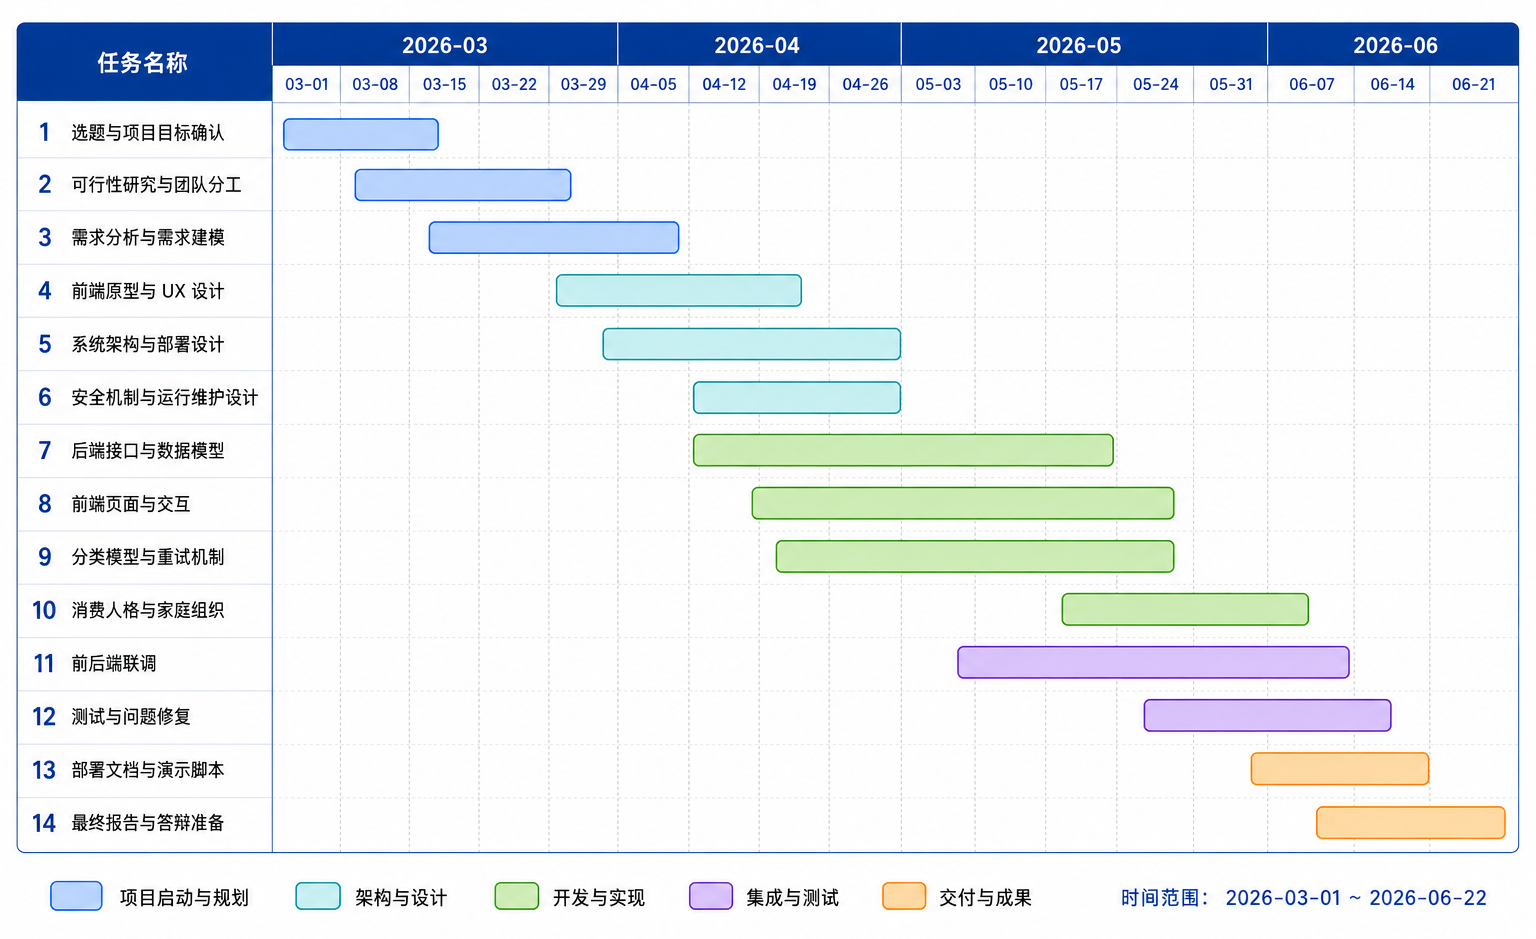
\includegraphics[width=0.92\textwidth]{简化甘特图.png}
  \caption{项目进度甘特图}
  \label{fig:gantt}
\end{figure}

\section{团队组织与协作}

\subsection{团队成员与分工}

项目由四名成员协作完成，各成员依据技术专长承担主要职责，并通过文档和规范降低人员交接成本。成员分工如表~\ref{tab:team} 所示。

\begin{table}[H]
\centering
\caption{团队成员与分工}
\label{tab:team}
\begin{tabular}{p{2cm}p{5.5cm}p{5.7cm}}
\toprule
\textbf{成员} & \textbf{主要职责} & \textbf{备份与协作机制} \\
\midrule
郑博文 & 项目管理、需求统筹、答辩材料整理 & 维护进度计划和课程要求对照表，协调文档合并与版本管理。 \\
\addlinespace
林子尧 & 后端开发、数据库设计、接口实现 & 通过接口文档和自动化测试用例降低后端代码的交接成本。 \\
\addlinespace
单彬 & 前端页面、交互流程、图表展示 & 通过组件拆分和统一的 API 客户端封装降低前端页面的维护成本。 \\
\addlinespace
沈柔希 & 分类模型、测试、部署与联调 & 维护分类策略配置、测试流程和部署脚本，确保模型处理流程和部署方案可复现。 \\
\bottomrule
\end{tabular}
\end{table}

\subsection{人员变动预案}

为应对开发过程中可能出现的人员变动风险，团队制定了表~\ref{tab:personnel-contingency} 所示的应急预案。

\begin{table}[H]
\centering
\caption{人员变动应急预案}
\label{tab:personnel-contingency}
\begin{tabular}{p{3.2cm}p{10cm}}
\toprule
\textbf{风险场景} & \textbf{应对方式} \\
\midrule
某成员生病或临时缺席 & 通过 Git 提交记录、接口文档和任务拆分让其他成员接手其负责模块的小范围修复工作。 \\
\addlinespace
某模块开发严重滞后 & 优先保证最小可行版本的核心业务流程可演示，暂缓模块内的增强功能，待核心流程稳定后再补充。 \\
\addlinespace
答辩前关键资料缺失 & 以 README、项目文档、汇报 PPT 和测试结果作为可追溯的证据链，确保交付物完整性。 \\
\bottomrule
\end{tabular}
\end{table}

\subsection{协作机制}

团队协作依托以下工程实践：

\begin{itemize}
  \item \textbf{版本控制}：使用 Git 进行代码版本管理，代码变更经过合并审查后进入主分支，以保持主分支可运行。
  \item \textbf{接口约定}：前后端以开放式接口规范（OpenAPI）文档为契约，后端接口变更需同步更新文档，前端基于接口文档独立开发。
  \item \textbf{每日同步}：通过即时通讯工具保持进度同步，关键设计决策通过集中讨论确定并记录在项目文档中。
  \item \textbf{文档持续化}：需求、设计、测试和部署等各阶段文档随开发过程持续撰写和更新，避免期末集中整理。
\end{itemize}

\section{风险管理}

项目启动阶段对主要风险进行了识别和评估，并制定了相应的缓解措施。风险矩阵如表~\ref{tab:risk-matrix} 所示。

\begingroup
\small
\begin{longtable}{p{3.2cm}p{1.2cm}p{1.2cm}p{1.2cm}p{6.4cm}}
\caption{项目风险矩阵}
\label{tab:risk-matrix}\\
\toprule
\textbf{风险} & \textbf{概率} & \textbf{影响} & \textbf{等级} & \textbf{缓解措施} \\
\midrule
\endfirsthead
\multicolumn{5}{c}{\small 表~\thetable\quad 项目风险矩阵（续）} \\
\toprule
\textbf{风险} & \textbf{概率} & \textbf{影响} & \textbf{等级} & \textbf{缓解措施} \\
\midrule
\endhead
\midrule
\multicolumn{5}{r}{\small 接下页} \\
\endfoot
\bottomrule
\endlastfoot
微信、支付宝账单格式差异 & 高 & 中 & 高 & 通过统一的平台识别与解析机制处理多种账单格式，使不同解析过程输出一致的交易结构，并保留测试样例。 \\
\addlinespace
大模型分类结果不稳定 & 中 & 中 & 中 & 在交易详情中展示分类理由和置信度；保留规则分类后备方案和分类缓存；低置信度交易进入人工校正队列。 \\
\addlinespace
外部模型 API 不可用或延迟高 & 中 & 中 & 中 & 支持本地模型服务；外部请求通过统一重试队列处理，多次失败后停止自动尝试，并可切换为规则分类。 \\
\addlinespace
家庭组织权限配置错误 & 中 & 高 & 高 & 使用组织成员角色校验，区分所有者、管理员和普通成员；个人账本默认不受组织功能影响；所有组织操作均校验成员身份。 \\
\addlinespace
后期时间不足 & 中 & 高 & 高 & 坚持最小可行产品优先策略，先保证核心业务流程可运行，再补充增强功能和文档润色。 \\
\addlinespace
多人协作接口不一致 & 中 & 中 & 中 & 以 OpenAPI 文档为前后端契约；后端测试覆盖核心接口；使用类型定义和统一通信层约束前端请求。 \\
\addlinespace
安全设计不足 & 中 & 高 & 高 & 使用 JWT 身份鉴别、密码摘要存储和资源归属校验；后续安全章节中列出已知改进项和加固建议。 \\
\addlinespace
大文件导入性能不足 & 中 & 中 & 中 & 当前限制上传文件规模；后续可通过异步任务、批量写入和数据库聚合查询优化大批量数据处理性能。 \\
\end{longtable}
\endgroup

\subsection{变更管理策略}

在迭代开发过程中，各类变更按照表~\ref{tab:change-management} 所示的策略进行处理，以确保变更不会影响核心业务流程的稳定性。

\begin{table}[H]
\centering
\caption{变更管理策略}
\label{tab:change-management}
\begin{tabular}{p{3cm}p{10.2cm}}
\toprule
\textbf{变更类型} & \textbf{处理方式} \\
\midrule
新增功能需求 & 先判断是否影响最小可行产品的核心业务流程；若不影响则放入后续增强列表，优先保证当前阶段交付。 \\
\addlinespace
接口字段变化 & 后端更新自动生成的 OpenAPI 接口规范，前端同步修改通信层和类型定义。 \\
\addlinespace
家庭组织权限变化 & 先保证个人账本默认行为不变，在此基础上扩展家庭聚合查询的权限校验逻辑。 \\
\addlinespace
分类策略变化 & 保留规则后备方案，记录每次分类的来源、置信度和分类理由，确保分类过程可追溯。 \\
\addlinespace
页面交互变化 & 优先不破坏主流程（导入→分类→分析→报表），避免在交付前进行大范围 UI 改版。 \\
\addlinespace
部署环境变化 & 同时维护本地直接启动和 Docker Compose 两套方案，保障在任何环境下系统均可演示。 \\
\bottomrule
\end{tabular}
\end{table}

\chapter{需求分析}

\section{需求获取方法}

本系统的需求通过五种方法获取，覆盖从用户行为分析到工程质量审查的完整链路。

\textbf{真实账单处理流程分析}：项目启动阶段，团队收集支付宝与微信支付的原始账单文件，模拟用户从下载账单、整理数据到生成报表的完整操作流程，提炼出导入、解析、分类、分析、报表五大核心环节，作为功能需求的主要依据。

\textbf{小组讨论与范围界定}：团队依据开发周期与技术能力，对需求进行优先级排序，将核心闭环（认证、导入、分类、分析、报表）确定为最高优先级，将消费人格分析、家庭组织、模型切换等纳入扩展范围，形成清晰的 MVP 边界。

\textbf{误分类案例分析}：团队收集了多种语义误判场景——如“东南大学饭卡充值”被通用分类归为“学习”、连锁便利店消费被归为“购物”而非“餐饮”——驱动了大模型初分、分类理由展示和人工校正工作台的需求。系统需在给出分类建议的同时，提供置信度与推理理由，允许用户在校正工作台中批量修正。

\textbf{原型与联调反馈}：在前后端迭代过程中，前端页面的交互细节和后端接口的返回结构经过多轮联调调整。例如，导入页面的进度轮询机制、校正工作台的左右分栏布局、家庭组织的角色权限控制，均来自原型验证阶段的反馈。

\textbf{工程质量审查}：团队对照安全、隐私、性能、可部署性、可维护性、可测试性等质量维度，识别并补齐非功能需求。这一步骤确保系统不仅是功能可用的原型，也是具备工程质量的交付物。

\headingneedspace{19}
\section{利益相关者分析}

系统涉及四类利益相关者，其关注点与需求来源如表所示。

\begin{table}[H]
\centering
\caption{利益相关者分析}
\label{tab:stakeholders}
\begin{tabular}{p{3.2cm} p{5.2cm} p{5.2cm}}
\toprule
\textbf{利益相关者} & \textbf{关注点} & \textbf{需求来源} \\
\midrule
普通用户 & 上传账单、查看 AI 分类结果、修正语义误判、查看消费画像、生成报表 & 个人记账与财务分析场景 \\
\hline
家庭组织管理员 & 创建家庭组织、添加成员、管理角色、查看家庭聚合分析 & 家庭账本协作场景 \\
\hline
系统运维人员 & 配置模型供应商、管理重试队列、部署与监控系统 & 系统部署与运维场景 \\
\hline
开发与维护人员 & 实现系统功能、控制开发范围、维护代码质量、准备后续扩展 & 工程开发与维护过程 \\
\bottomrule
\end{tabular}
\end{table}

\section{功能需求}

系统共识别 15 项功能需求，按优先级分为 P0（核心闭环必备）、P1（完整性与体验增强）和 P2（未来改进）。当前实现覆盖全部 P0 与 P1 需求。

\begingroup
\small
\begin{longtable}{p{1.0cm} p{3.5cm} p{0.8cm} p{6.2cm}}
\caption{功能需求列表}
\label{tab:functional-requirements}\\
\toprule
\textbf{ID} & \textbf{需求描述} & \textbf{优先级} & \textbf{实现依据} \\
\midrule
\endfirsthead
\multicolumn{4}{c}{\small 表~\thetable\quad 功能需求列表（续）} \\
\toprule
\textbf{ID} & \textbf{需求描述} & \textbf{优先级} & \textbf{实现依据} \\
\midrule
\endhead
\midrule
\multicolumn{4}{r}{\small 接下页} \\
\endfoot
\bottomrule
\endlastfoot
FR-01 & 用户注册、登录及 Token 鉴权 & P0 & \texttt{routes\_auth.py}、前端登录页、JWT 中间件 \\
\hline
FR-02 & 多用户数据隔离，账单与报表按用户归属 & P0 & \texttt{dependencies.py} 依赖注入、资源归属校验 \\
\hline
FR-03 & 支持微信/支付宝账单文件上传导入 & P0 & \texttt{routes\_imports.py}、导入页面 \\
\hline
FR-04 & 不同平台账单统一解析为标准化交易结构 & P0 & \texttt{services/parsers.py}、\texttt{test\_parsers.py} \\
\hline
FR-05 & 大模型语义分类，记录来源、置信度与理由 & P0 & \texttt{services/classifiers.py}、\texttt{test\_classifiers.py} \\
\hline
FR-06 & 交易列表筛选（日期、平台、分类、关键词）与分页 & P0 & \texttt{routes\_transactions.py}、交易列表页面 \\
\hline
FR-07 & 人工校正低置信度或语义误判交易 & P0 & \texttt{routes\_transactions.py} PATCH 接口、校正工作台 \\
\hline
FR-08 & 用户自定义分类管理 & P1 & \texttt{routes\_categories.py}、分类管理页面 \\
\hline
FR-09 & Dashboard 展示收入、支出、结余、储蓄率、分类占比 & P0 & \texttt{routes\_dashboard.py}、\texttt{services/analytics.py} \\
\hline
FR-10 & 消费人格画像、财务健康评分与问卷自评 & P1 & \texttt{routes\_personality.py}、\texttt{services/personality.py} \\
\hline
FR-11 & 家庭组织创建与成员角色管理 & P1 & \texttt{routes\_organizations.py}、\texttt{services/organizations.py} \\
\hline
FR-12 & 家庭组织 Dashboard 与消费人格聚合 & P1 & \texttt{organization\_id} 查询参数、组织页面 \\
\hline
FR-13 & PDF 报表生成与下载，支持个人与家庭模式 & P0 & \texttt{routes\_reports.py}、\texttt{services/reports.py} \\
\hline
FR-14 & 分类供应商切换（规则/外部 API/本地模型） & P1 & \texttt{services/classifiers.py} CompositeClassifier \\
\hline
FR-15 & 外部模型失败重试队列与管理员控制 & P1 & \texttt{routes\_classification.py}、\texttt{retry\_queue.py} \\
\end{longtable}
\endgroup

\headingneedspace{6}
FR-01 至 FR-07、FR-09、FR-13 构成系统的核心闭环：认证后导入账单并自动分类，经人工校对后产出 Dashboard 分析与 PDF 报表。FR-08、FR-10 至 FR-12、FR-14、FR-15 在此闭环上增加了消费人格画像、家庭协作和运维可控性。

\section{非功能需求}

系统定义了 8 项非功能需求，涵盖安全性、隐私保护、可用性、性能、可部署性、可维护性、可测试性与可扩展性。

\begin{table}[H]
\centering
\caption{非功能需求列表}
\label{tab:nfr}
\begin{tabular}{p{1.5cm} p{3cm} p{1cm} p{7.8cm}}
\toprule
\textbf{ID} & \textbf{需求名称} & \textbf{优先级} & \textbf{说明} \\
\midrule
NFR-01 & 安全性 & P0 & 密码采用哈希存储，业务接口均需 JWT 鉴权，资源访问按用户归属校验 \\
\hline
NFR-02 & 隐私保护 & P0 & 账单数据、分类结果与 PDF 报表属于敏感个人财务数据，用户间严格隔离 \\
\hline
NFR-03 & 可用性 & P0 & 用户可按“导入→初分→校正→分析→报表”路径完成核心任务；家庭功能不破坏个人模式 \\
\hline
NFR-04 & 性能 & P1 & 非模型调用接口（认证、查询、聚合分析）在单用户正常操作下 P95 响应时间应低于 1 秒；大模型分类调用设有 60 秒超时保护（\texttt{model\_timeout\_seconds=60}）与最多 2 次自动重试；≤1000 笔交易的单批次文件解析阶段应在 10 秒内完成，进度通过轮询接口实时反映 \\
\hline
NFR-05 & 可部署性 & P0 & 支持本地开发模式、Docker Compose 部署与裸机部署三种方式 \\
\hline
NFR-06 & 可维护性 & P0 & 前后端分离；后端按 routes/services/models/schemas 分层组织 \\
\hline
NFR-07 & 可测试性 & P0 & 后端具备 pytest 自动化测试套件，前端通过 TypeScript 类型检查与生产构建验证 \\
\hline
NFR-08 & 可扩展性 & P1 & 分类供应商、报表生成、异步任务与部署组件预留扩展接口 \\
\bottomrule
\end{tabular}
\end{table}

\section{用户场景分析}

\subsection{普通用户场景}

普通用户的核心场景覆盖“导入—分类—校正—分析—报表”的完整链路：

\begin{enumerate}
  \item 用户注册账号并登录系统，进入应用主界面。
  \item 进入账单导入页面，上传微信或支付宝账单文件（CSV 格式）。
  \item 系统创建导入批次，后台解析账单并将不同平台格式转换为统一交易记录。
  \item 系统调用大模型对每条交易进行语义初分，记录分类来源、置信度与分类理由。
  \item 用户在交易列表中按日期、平台、分类、关键词筛选查看交易。
  \item 在分类校正工作台中，用户查看待校正交易队列，对低置信度或语义误判的分类进行人工修正。
  \item 用户进入 Dashboard 查看收入支出概览、储蓄率、分类占比图与 Top 商户。
  \item 用户进入消费人格页面，查看基于交易数据计算的消费人格画像、财务健康评分，并可通过问卷进行自评对比。
  \item 用户进入报表中心，选择日期范围与导入文件，生成并下载 PDF 报表。
\end{enumerate}

\subsection{家庭组织场景}

家庭组织场景描述管理员创建家庭、管理成员并查看聚合分析的过程：

\begin{enumerate}
  \item 用户创建家庭组织，系统自动将创建者设为 owner 角色。
  \item owner 或 admin 通过用户名搜索添加成员，并可提升普通成员为 admin。
  \item 家庭成员进入组织页面查看家庭合计收入、支出、交易数与消费人格聚合雷达图。
  \item owner 或 admin 可触发家庭范围内的重分类操作；普通 member 只能查看聚合结果。
  \item 不传入 \texttt{organization\_id} 参数时，Dashboard、Personality 和 Reports 仍按个人账本模式工作，保持向后兼容。
\end{enumerate}

\subsection{系统运维场景}

运维人员关注系统部署、配置与故障恢复：

\begin{enumerate}
  \item 运维人员配置后端运行环境，包括数据库连接、Redis 缓存、模型供应商与 API 密钥。
  \item 部署前端静态资源、Nginx 反向代理、FastAPI 后端、PostgreSQL 与 Redis。
  \item 当模型请求超时或失败时，运维人员通过重试状态接口查看队列中的交易数量与供应商分布。
  \item 运维人员通过管理界面将历史超时或失败交易重新放入重试队列，恢复分类流程。
\end{enumerate}

\section{异常场景处理}

系统对以下异常场景定义了明确的预期行为：

\begin{table}[H]
\centering
\caption{异常场景与系统预期行为}
\label{tab:exception-scenarios}
\begin{tabular}{p{4.8cm} p{8.5cm}}
\toprule
\textbf{异常场景} & \textbf{系统预期行为} \\
\midrule
用户未登录访问业务接口 & 返回 401 未授权状态码，前端跳转至登录页 \\
\hline
用户上传不支持的账单格式 & 导入失败并记录具体错误信息，页面提示用户重新上传 \\
\hline
重复导入同一笔交易 & 通过 \texttt{dedupe\_hash} 字段去重，避免重复记录入库 \\
\hline
模型供应商不可用 & 交易进入重试队列，后台串行重试；超时耗尽后标记为 retry\_failed \\
\hline
用户尝试访问他人报表或交易 & 后端按 \texttt{current\_user.id} 校验资源归属，拒绝非授权访问 \\
\hline
报表生成失败 & 记录任务状态与错误信息，用户可调整参数后重新触发生成 \\
\bottomrule
\end{tabular}
\end{table}

\section{用例建模}

系统用例图展示三类参与者（普通用户、家庭管理员、系统运维人员）与系统功能之间的关系。普通用户可操作认证、导入、查看交易、校正分类、管理自定义分类、查看 Dashboard、生成报表、查看消费人格等用例；家庭管理员额外可创建组织和管理成员；系统运维人员负责供应商配置与重试队列管理。导入账单用例包含大模型语义分类作为扩展关系。

\begin{figure}[H]
  \centering
  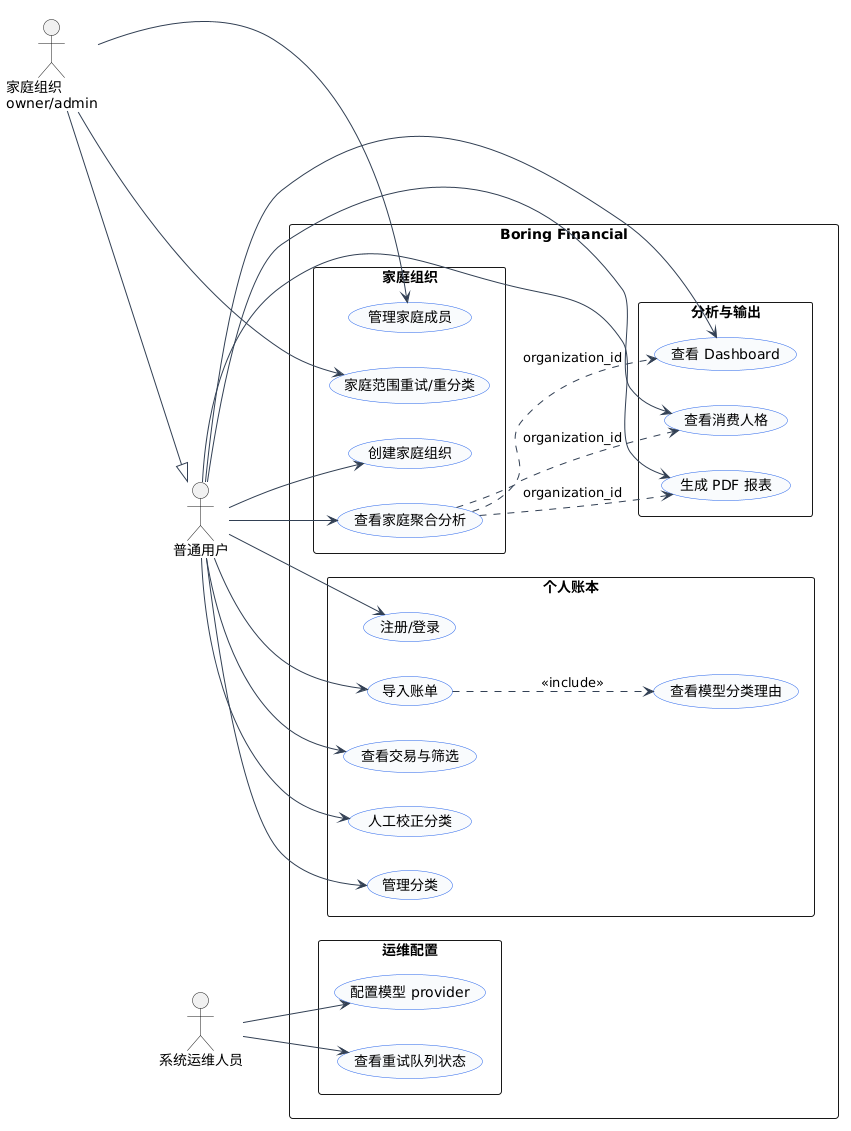
\includegraphics[width=0.92\textwidth]{用例图.png}
  \caption{系统用例图}
  \label{fig:usecase}
\end{figure}

\section{用例规约}

以下对两个核心用例给出结构化用例说明，包含基本流程、替代流程与异常流程。

\subsection{UC-01：导入账单与语义分类}

\begin{table}[H]
\centering
\caption{用例规约：导入账单与语义分类}
\label{tab:uc01}
\small
\begin{tabular}{p{2.8cm} p{10.5cm}}
\toprule
\textbf{用例名称} & 导入账单与语义分类 \\
\midrule
\textbf{参与者} & 普通用户（主）；大模型分类服务（外部系统） \\
\hline
\textbf{触发条件} & 用户进入账单导入页面，选择账单文件并点击上传 \\
\hline
\textbf{前置条件} & 用户已登录；待上传文件为微信或支付宝 CSV 格式 \\
\hline
\textbf{后置条件} & 交易记录入库完毕，语义初分完成，批次状态置为 \texttt{done} 或 \texttt{partial\_failed} \\
\hline
\textbf{基本流程} &
1）用户拖拽或选择账单文件。\newline
2）前端调用 \texttt{POST /api/imports} 上传文件内容。\newline
3）系统创建 \texttt{ImportBatch}，将原始文件写入磁盘。\newline
4）后台线程解析 CSV，将各平台格式转换为统一 \texttt{Transaction} 结构。\newline
5）对每笔新交易计算 \texttt{dedupe\_hash}，跳过已存在的重复记录。\newline
6）调用 \texttt{CompositeClassifier}（缓存→外部 API→本地模型→规则回退）进行语义分类，结果写入 \texttt{auto\_category\_id}、\texttt{auto\_confidence}、\texttt{auto\_reason}。\newline
7）批次状态更新为 \texttt{done}，前端轮询后展示完成提示。\\
\hline
\textbf{替代流程 A} & 部分交易模型超时（超过 60 秒）：失败交易标记为 \texttt{retry\_queue}，其余交易正常入库，批次状态置为 \texttt{partial\_failed}。 \\
\hline
\textbf{替代流程 B} & 文件含已导入交易：\texttt{dedupe\_hash} 自动去重，跳过重复记录，批次仍正常完成。 \\
\hline
\textbf{异常流程} & 文件格式无法识别（非微信／支付宝 CSV）：文件状态标记为 \texttt{failed}，错误信息写入 \texttt{error\_message}，页面提示用户重新上传。 \\
\bottomrule
\end{tabular}
\end{table}

\subsection{UC-02：人工校正分类结果}

\begin{table}[H]
\centering
\caption{用例规约：人工校正分类结果}
\label{tab:uc02}
\small
\begin{tabular}{p{2.8cm} p{10.5cm}}
\toprule
\textbf{用例名称} & 人工校正分类结果 \\
\midrule
\textbf{参与者} & 普通用户 \\
\hline
\textbf{触发条件} & 用户进入分类校正工作台 \\
\hline
\textbf{前置条件} & 系统中存在 \texttt{needs\_review=true} 的交易记录 \\
\hline
\textbf{后置条件} & 目标交易的 \texttt{final\_category\_id} 已更新，\texttt{needs\_review} 置为 \texttt{false}，校正结果实时反映在 Dashboard 及报表数据中 \\
\hline
\textbf{基本流程} &
1）前端加载待校正队列（\texttt{needs\_review=true}，按置信度升序排列）。\newline
2）用户选中一笔交易，右侧面板展示商户、金额、当前分类、置信度与模型推理理由。\newline
3）用户从系统分类或自定义分类中选择正确类别，点击"确认校正"。\newline
4）前端调用 \texttt{PATCH /api/transactions/\{id\}}，提交新的 \texttt{final\_category\_id}。\newline
5）后端更新交易记录，将 \texttt{needs\_review} 置为 \texttt{false}。\newline
6）前端从待校正队列移除该交易，自动加载下一笔。\\
\hline
\textbf{替代流程} & 用户认为当前分类正确：直接点击"确认当前分类"，后端同样将 \texttt{needs\_review} 置为 \texttt{false}，\texttt{final\_category\_id} 保留原 \texttt{auto\_category\_id}。 \\
\hline
\textbf{异常流程} & 所需自定义分类尚不存在：用户跳转至分类管理页面新增分类后，返回工作台重新操作。 \\
\bottomrule
\end{tabular}
\end{table}

\section{业务流程建模}

核心业务活动图描述了从用户登录到报表生成的端到端流程。流程始于用户登录，接着上传账单文件，系统创建导入批次后进行解析和去重；成功解析的交易经过大模型语义初分，高置信度结果直接入库，低置信度交易进入人工复核队列；用户完成校正后，交易数据进入 Dashboard 聚合分析，随后流向消费人格与财务健康分析模块；在报表生成环节，系统根据是否选择家庭组织参数，分别生成个人 PDF 报表或家庭聚合 PDF 报表。

\begin{figure}[!htbp]
  \centering
  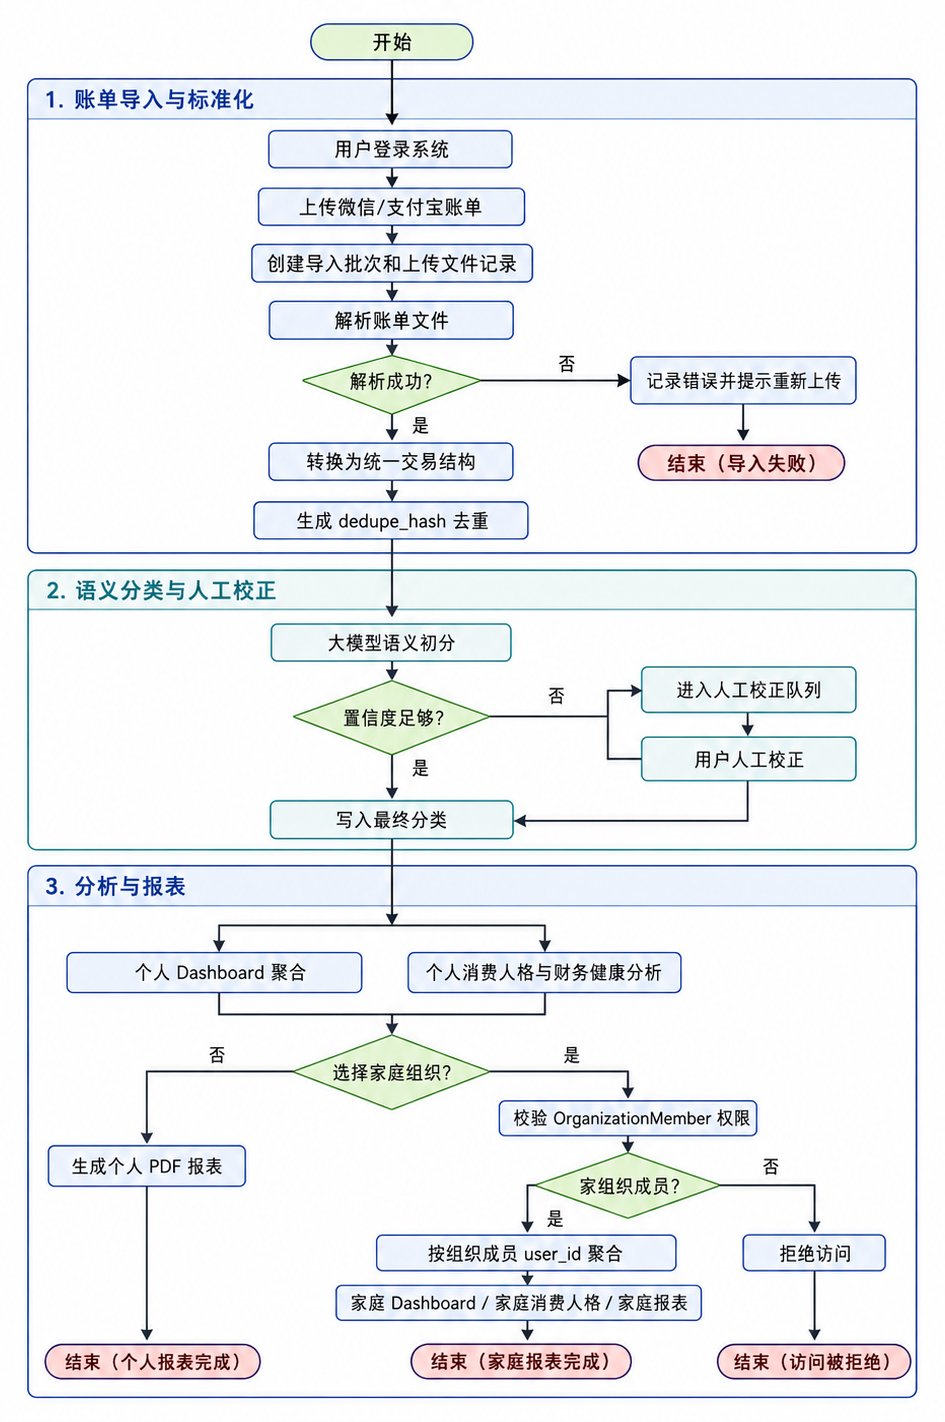
\includegraphics[
    width=0.58\textwidth,
    height=0.47\textheight,
    keepaspectratio
  ]{核心业务活动图.png}
  \caption{核心业务活动图}
  \label{fig:activity}
\end{figure}

\chapter{用户界面与体验设计}

\section{设计迭代过程}

系统 UI 设计随开发迭代同步演进，经历以下三个阶段。

\textbf{第一阶段——场景驱动草图}：需求分析阶段，团队依据普通用户、家庭管理员、运维人员三类场景，推演各页面的核心信息与操作动线，确定整体布局框架：深色侧边栏承载全局导航，白色卡片区承载数据展示。各功能页面的布局模式在此阶段确定：Dashboard 采用摘要卡片组加图表区的双层结构；校正工作台采用左侧队列加右侧详情的双栏分割；交易列表采用顶部筛选栏加分页表格。

\textbf{第二阶段——设计系统建立}：首个开发迭代中，以 Dashboard 页面为标准件，确定色板、字号层级与间距规范，检验组件复用与色彩层级的一致性，形成贯穿全系统的设计语言（详见下节"设计系统"）。

\textbf{第三阶段——联调反馈与细节调整}：前后端联调过程中，交互细节根据真实操作反馈迭代调整。导入页面的进度展示方式、校正工作台的双栏布局与队列排序逻辑、家庭组织页面的角色权限控件可见性，均在多轮联调中根据反馈完善，最终形成本章所展示的页面形态。

\section{设计系统}

系统采用专业金融工具风格的设计体系，以深色导航与浅色内容区形成清晰的视觉层级。设计系统的核心参数如下：

\begin{table}[H]
\centering
\caption{设计系统色板}
\label{tab:design-system}
\begin{tabular}{p{3.5cm} p{3.5cm} p{3.5cm}}
\toprule
\textbf{色板角色} & \textbf{色值} & \textbf{应用位置} \\
\midrule
深色侧边栏底色 & \texttt{\#06233D} & 左侧导航栏背景 \\
\hline
深色侧边栏悬浮色 & \texttt{\#041A2E} & 导航项悬停/选中态 \\
\hline
品牌主色 & \texttt{\#00A884} & 主要按钮、链接、数据高亮 \\
\hline
页面背景 & \texttt{\#F5F7FA} & 内容区域整体背景 \\
\hline
卡片背景 & \texttt{\#FFFFFF} & 数据卡片、表格、表单容器 \\
\hline
成功色 & \texttt{\#22C55E} & 成功状态、收入标识 \\
\hline
警告色 & \texttt{\#F59E0B} & 警告提示、中等置信度 \\
\hline
错误色 & \texttt{\#EF4444} & 错误状态、支出标识 \\
\hline
信息色 & \texttt{\#3B82F6} & 信息提示、链接、进度条 \\
\bottomrule
\end{tabular}
\end{table}

深色侧边栏提供全局导航，顶部栏显示当前页面标题与用户信息区域。主内容区采用白色卡片承载数据面板、表格与表单，通过规则间距与统一圆角保持视觉一致性。图表采用 ECharts 渲染，配色与设计系统色板保持一致，确保图表与页面风格协调。

\section{主要页面原型}

系统共设计 10 个主要页面，本节逐一描述各页面的功能定位与关键交互。

\subsection{登录与注册页面}

登录与注册页面采用左右分栏布局：左侧为深色品牌展示区，包含应用名称与简短说明；右侧为白色表单卡片，包含用户名与密码输入框，以及登录与注册模式切换按钮。注册模式额外显示邮箱字段。验证成功后，用户进入系统主界面。

\begin{figure}[H]
  \centering
  \uiscreenshot{截图-登陆注册页.png}
  \caption{登录与注册页面截图}
  \label{fig:screenshot-login}
\end{figure}

\subsection{仪表盘页面}

Dashboard 是系统的财务驾驶舱，顶部展示收入、支出、结余、储蓄率四张摘要卡片。中部为支出趋势折线图和分类占比饼图，右侧展示 Top 商户排行榜。用户可通过顶部日期筛选器切换统计周期，从整体趋势快速定位异常支出。

\begin{figure}[H]
  \centering
  \uiscreenshot{截图-dashboard.png}
  \caption{仪表盘页面截图}
  \label{fig:screenshot-dashboard}
\end{figure}

\clearpage
\subsection{账单导入页面}

账单导入页面提供拖拽上传区域，支持微信与支付宝 CSV 账单文件。上传成功后，页面展示最近导入记录列表，包含文件名、平台、状态与处理进度条，支持批量进度轮询。用户可点击导入记录查看详情，或删除历史导入批次。

\begin{figure}[H]
  \centering
  \uiscreenshot{截图-导入账单.png}
  \caption{账单导入页面截图}
  \label{fig:screenshot-import}
\end{figure}

\subsection{交易列表页面}

交易列表页面以筛选栏加分页表格的形式展示所有交易记录。筛选条件包括日期范围、平台（微信/支付宝）、分类、导入文件和关键词搜索。表格每行显示时间、商户、金额、分类与置信度。点击行可展开详情抽屉，展示分类来源、置信度、分类理由与原始交易备注。

\begin{figure}[H]
  \centering
  \uiscreenshot{截图-交易列表.png}
  \caption{交易列表页面截图}
  \label{fig:screenshot-transactions}
\end{figure}

\clearpage
\subsection{分类校正工作台}

校正工作台采用左右分栏布局：左侧为待校正交易队列，按置信度从低到高排序，每项显示商户、金额与当前分类；右侧为当前选中交易的详细信息，包括模型分类建议（来源、置信度、推理理由），以及分类选择控件，允许用户选择新的系统分类或自定义分类并确认修正。确认后交易从队列中移除。

\begin{figure}[H]
  \centering
  \uiscreenshot{截图-分类矫正.png}
  \caption{分类校正工作台截图}
  \label{fig:screenshot-review}
\end{figure}

\subsection{分类管理页面}

分类管理页面展示系统预设分类与用户自定义分类。顶部为分类使用频率统计，按交易数量排序。中部为分类列表，系统分类标记为锁定不可删除，用户自定义分类支持新增、编辑与禁用操作。修改操作通过弹窗表单完成，实时生效。

\begin{figure}[H]
  \centering
  \uiscreenshot{截图-分类管理.png}
  \caption{分类管理页面截图}
  \label{fig:screenshot-categories}
\end{figure}

\clearpage
\subsection{消费人格页面}

消费人格页面由三个区域组成：顶部为 16 型消费人格画像卡片，展示用户所属人格类型及简要描述；中部为四维雷达图（现时偏好、心理账户、炫耀性消费、开放性），展示各维度得分；底部为财务健康评分区域，展示储蓄率、收入稳定性、消费多样性、支出波动性和应急能力的子指标。页面同时提供问卷自评入口，用户可对比主观认知与交易数据画像的偏差。

\begin{figure}[H]
  \centering
  \uiscreenshot{截图-消费人格.png}
  \caption{消费人格页面截图}
  \label{fig:screenshot-personality}
\end{figure}

\subsection{家庭组织页面}

家庭组织页面在用户未加入任何组织时显示创建引导。已有组织时，页面展示三部分内容：左侧为成员列表，每行显示用户名、角色与管理按钮；右上方为家庭财务概览卡片，展示组织合计收入、支出与交易数；右下方为家庭消费人格聚合雷达图，将所有成员交易数据按人格维度聚合展示。家庭所有者和管理员可见角色管理控件与重分类触发按钮。

\begin{figure}[H]
  \centering
  \uiscreenshot{截图-家庭组织.png}
  \caption{家庭组织页面截图}
  \label{fig:screenshot-organization}
\end{figure}

\clearpage
\subsection{报表中心页面}

报表中心页面提供日期范围选择器与导入文件筛选器。用户设置条件后点击生成按钮，系统异步创建报表任务。生成完成后，页面展示报表摘要信息（覆盖时间段、交易数、分类分布），并提供 PDF 下载按钮。历史报表列表按生成时间倒序排列，支持重新下载。

\begin{figure}[H]
  \centering
  \uiscreenshot{截图-报表中心.png}
  \caption{报表中心页面截图}
  \label{fig:screenshot-reports}
\end{figure}

\subsection{系统设置页面}

系统设置页面向所有用户展示当前分类供应商名称、置信度阈值等配置信息。管理员用户额外可见重试队列控制区：包括当前队列状态（等待重试数、重试中数、已失败数），以及“一键重试历史超时”按钮。普通用户仅可见配置展示，管理操作控件隐藏。

\begin{figure}[H]
  \centering
  \uiscreenshot{截图-系统设置.png}
  \caption{系统设置页面截图}
  \label{fig:screenshot-settings}
\end{figure}

\section{界面信息架构与交互组织}

系统界面围绕“全局导航、任务页面、状态反馈、数据可视化”四类信息组织。该划分使用户在不同业务页面之间切换时保持一致的认知模型，也便于后续新增功能时复用相同的交互规则。

\begin{table}[H]
\centering
\caption{界面信息架构与交互组织}
\label{tab:frontend-components}
\begin{tabular}{p{4.5cm} p{9cm}}
\toprule
\textbf{界面区域} & \textbf{设计职责} \\
\midrule
全局导航 & 以深色侧边栏承载主要功能入口，保证用户可在导入、交易、校正、分析、报表等任务之间快速切换 \\
\hline
页面标题与用户区 & 在顶部区域展示当前任务语境、用户身份和必要操作，减少用户对当前位置的判断成本 \\
\hline
任务主区域 & 各页面按“筛选—列表—详情”或“概览—图表—明细”的结构组织内容，匹配财务数据查看和校正流程 \\
\hline
状态反馈 & 导入、报表生成和模型重试等耗时任务通过进度、状态标签和结果摘要展示处理进展 \\
\hline
权限可见性 & 管理员功能、家庭角色管理和普通用户配置展示在界面上区分可见，避免误操作 \\
\hline
数据可视化 & 看板、人格画像和家庭聚合页面采用图表表达趋势、占比和维度评分，辅助用户理解财务状态 \\
\bottomrule
\end{tabular}
\end{table}

交互组织上，系统将身份状态、当前组织和页面筛选条件保持为跨页面可感知的上下文。用户切换页面后不需要重复登录或重新理解导航结构；需要管理员权限的操作仅在具备权限时出现，普通用户界面保持简洁。

\section{用户体验目标}

系统用户体验设计围绕以下四个核心目标展开：

\textbf{减少用户操作步骤}：账单导入采用拖拽上传模式，一次上传即可触发解析→去重→分类的全自动链路。Dashboard 与人格页面的数据通过后端聚合计算，用户无需手动维护分类映射表或公式。批量校正工作台允许用户在单一页面完成所有低置信度交易的复核，无需逐条跳转。

\textbf{分类结果可解释、可校正}：模型分类结果不仅给出类别，还提供置信度与人类可读的推理理由。校正工作台将模型建议与修改控件并置，用户可在了解 AI 推理过程后做出校正决策。校正结果即时生效，无需额外保存步骤。

\textbf{校正数据全链路贯通}：人工校正后的交易分类应实时反映在 Dashboard 聚合、消费人格计算和 PDF 报表中。系统通过统一数据源（transactions 表）确保各分析模块使用一致的最新分类结果，避免出现“已校正但图表未更新”的不一致情况。

\textbf{个人模式不受家庭功能影响}：家庭组织功能采用显式 opt-in 设计——用户需主动创建或加入组织，并在看板和报表页面主动切换至家庭视图。未切换时，所有页面保持个人账本模式，确保现有用户的体验不受影响。

\chapter{系统设计}

本章阐述\projectname 的架构设计，涵盖架构驱动因素、总体运行时结构、技术选型、模块职责、数据隔离、部署方案以及安全机制。

\section{架构驱动因素与设计原则}

架构设计并非从技术栈出发，而是由第 3 章的功能需求和质量场景共同驱动。系统最重要的架构目标如下：

\begin{enumerate}
  \item \textbf{财务数据默认隔离}：认证后的所有私有资源访问必须绑定当前用户；家庭聚合需要显式组织参数与成员身份校验。
  \item \textbf{分类结果可解释、可修正}：自动分类必须保留分类来源、置信度和理由，人工确定的最终分类不得被后续自动分类覆盖。
  \item \textbf{外部模型故障不阻塞核心业务流程}：导入、交易查看和人工校正不能依赖模型服务持续在线；超时请求进入统一重试机制。
  \item \textbf{变化点可替换}：新增账单平台或分类服务提供方时，应尽量限制修改范围，不影响交易、财务看板和报表能力。
  \item \textbf{轻量运行与工程化部署并存}：开发或演示环境可使用 SQLite 和应用内任务，容器化环境可使用 PostgreSQL、Redis 和独立后台任务处理器。
\end{enumerate}

据此采用模块化、分层、接口契约优先、用户数据默认隔离、外部能力可降级和部署能力可裁剪六项设计原则。系统属于\textbf{前后端分离的模块化单体应用}：后端业务模块运行在同一个 FastAPI 应用中，并通过接口层、业务层、数据层和基础设施层控制耦合；它不是按业务域独立部署的微服务系统。

\section{总体架构}

系统运行时结构分为展示层、接入层、应用层、异步处理层以及数据与外部服务层。

\begin{enumerate}
  \item \textbf{展示层}：Vue 3 + Element Plus + ECharts 构建的单页应用，运行于用户浏览器，负责全部用户交互与数据可视化。
  \item \textbf{接入层}：生产环境使用 Nginx 提供静态文件服务与反向代理，开发环境由前端开发服务器完成同源转发。
  \item \textbf{应用层}：FastAPI 接口层处理 HTTP 请求、身份校验和数据转换，业务层实现导入、分类、聚合、组织和报表逻辑。
  \item \textbf{异步处理层}：重试任务处理器随应用启动，依次处理外部模型请求；Celery 提供可选的独立任务执行能力，用于需要与请求过程分离的导入、重分类或报表任务。
  \item \textbf{数据与外部服务层}：PostgreSQL（生产）或 SQLite（轻量部署）存储业务数据，Redis 支持可选的任务队列，文件存储保存上传账单与 PDF；分类服务可以是外部兼容接口或本地模型服务。
\end{enumerate}

\begin{figure}[H]
  \centering
  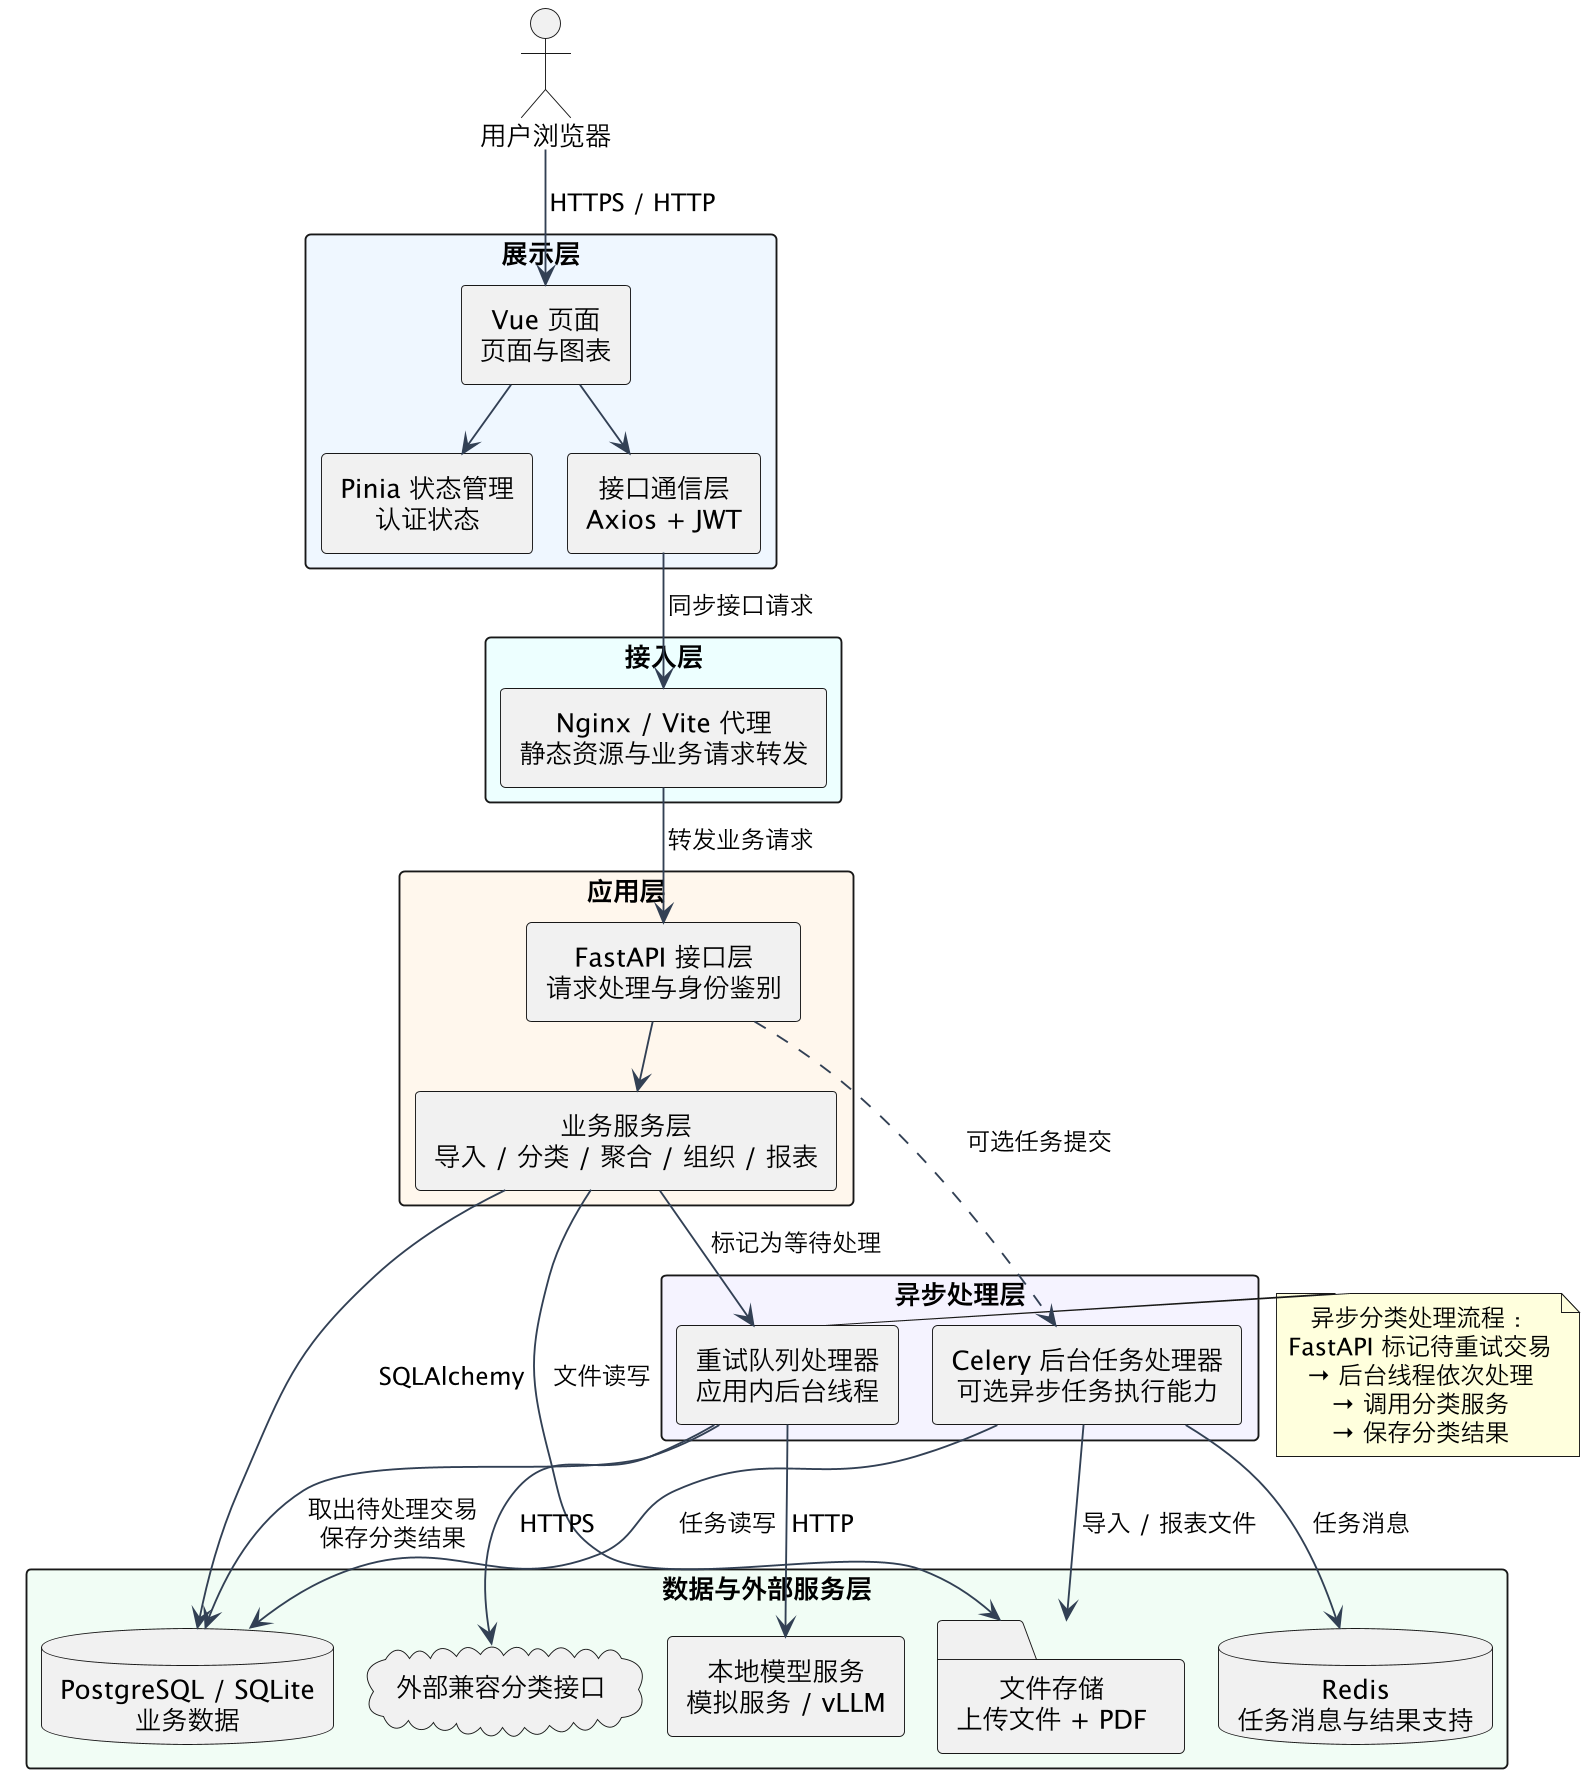
\includegraphics[width=0.88\textwidth,height=0.78\textheight,keepaspectratio]{architecture-overview.png}
  \caption{系统总体运行时架构图}
  \label{fig:architecture}
\end{figure}

图~\ref{fig:architecture} 中，同步请求沿“浏览器→前端→接入层→FastAPI→数据库或文件存储”流转；外部模型分类采用“业务服务记录待处理交易→后台任务处理器取出任务→调用分类服务→保存结果”的独立处理流程。该图只描述运行时构件，模块依赖与物理部署分别由组件图、包图和部署图表达。

\begin{table}[H]
\centering
\small
\caption{关键架构决策}
\label{tab:architecture-decisions}
\begin{tabularx}{0.98\textwidth}{p{2.7cm} p{3.5cm} X p{3.2cm}}
\toprule
\textbf{决策} & \textbf{需求来源} & \textbf{实现及理由} & \textbf{代价与限制} \\
\midrule
前后端分离的模块化单体 & 多页面交互、可维护性与轻量部署 & Vue 与 FastAPI 通过表述性状态转移应用程序接口（REST API）通信；后端按业务模块和分层目录组织，部署单元保持简单 & 不能像微服务一样按业务模块独立扩缩容 \\
\hline
统一交易结构 & FR-03、FR-04、可扩展性场景 & 将平台差异封装在解析模块中，对下游提供统一交易数据 & 新平台仍需补充列映射和测试样例 \\
\hline
复合分类与统一输出 & FR-05、FR-14 & 缓存、模型和规则采用统一结果结构，其他模块不需要了解分类服务差异 & 分类过程和状态比单一规则复杂 \\
\hline
后台重试机制 & FR-15、模型超时场景 & 数据库记录等待任务，后台处理器依次执行并采用指数退避，避免短时间大量重复请求 & 单实例处理能力有限，多实例运行时需要进一步协调 \\
\hline
自动/最终双分类字段 & FR-07、结果可追溯性 & 自动建议与人工决定分开保存，统计优先使用最终分类 & 查询和更新需统一处理分类优先级 \\
\hline
个人归属 + 查询时家庭聚合 & FR-11、FR-12、数据隔离 & 交易始终归属个人，家庭视图通过成员 ID 集合聚合 & 聚合查询比直接绑定组织更复杂 \\
\hline
报表构建与任务记录 & FR-13 & 构建器模式分离数据准备与页面渲染，并记录报表处理状态 & 当前仍采用同步生成，大报表可能占用请求处理资源 \\
\bottomrule
\end{tabularx}
\end{table}

\section{技术选型}

下表列出各层采用的核心技术及其选型依据。

\begin{table}[H]
  \centering
  \caption{技术选型汇总}
  \label{tab:tech-selection}
  \begin{tabular}{@{}p{3.0cm} p{2.8cm} p{7.8cm}@{}}
    \toprule
    \textbf{技术} & \textbf{用途} & \textbf{选型依据} \\
    \midrule
    FastAPI（Python） & 后端 API 框架 & 原生异步支持，可自动生成 OpenAPI 文档，并通过数据模型完成请求与响应验证 \\
    \hline
    Vue 3 + TypeScript & 前端框架 & 组合式 API 支持高复用的逻辑组织，TypeScript 编译期类型检查降低运行时错误 \\
    \hline
    Element Plus & UI 组件库 & 成熟的 Vue 3 组件生态，提供表格、表单、弹窗、导航等企业级组件 \\
    \hline
    ECharts & 数据可视化 & 支持雷达图、柱状图、折线图、饼图等，满足财务看板与人格分析的可视化需求 \\
    \hline
    SQLAlchemy 2.x & ORM 框架 & Data Mapper 模式解耦领域逻辑与持久化，支持 SQLite/PostgreSQL 双数据库切换 \\
    \hline
    Celery + Redis & 可选异步任务队列 & 已定义导入、重分类和报表任务；容器化部署可启动独立后台任务处理器，Redis 提供消息传递与结果存储 \\
    \hline
    fpdf2 & PDF 生成 & 轻量级 Python PDF 库，无外部依赖，支持 Unicode 中文字体加载 \\
    \hline
    Docker Compose & 多服务部署 & 统一启动多个运行组件，降低不同环境之间的配置差异 \\
    \bottomrule
  \end{tabular}
\end{table}

\section{前端架构}

前端按职责划分为视图、状态、通信、导航和类型约束五个层次。视图层由 10 个页面构成，对应登录、财务看板、导入、交易列表、校正工作台、分类管理、消费人格、家庭组织、报表中心和系统设置；状态层管理认证状态与跨页面信息；通信层统一处理后台请求和身份凭证；导航层控制页面访问与按需加载；类型约束层统一描述前后台交换的数据结构。

前端视觉设计规范以深色导航（\texttt{\#06233D}）、品牌色（\texttt{\#00A884}）与浅灰页面背景（\texttt{\#F5F7FA}）构成统一视觉语言，详见第 4 章。

\begin{figure}[H]
  \centering
  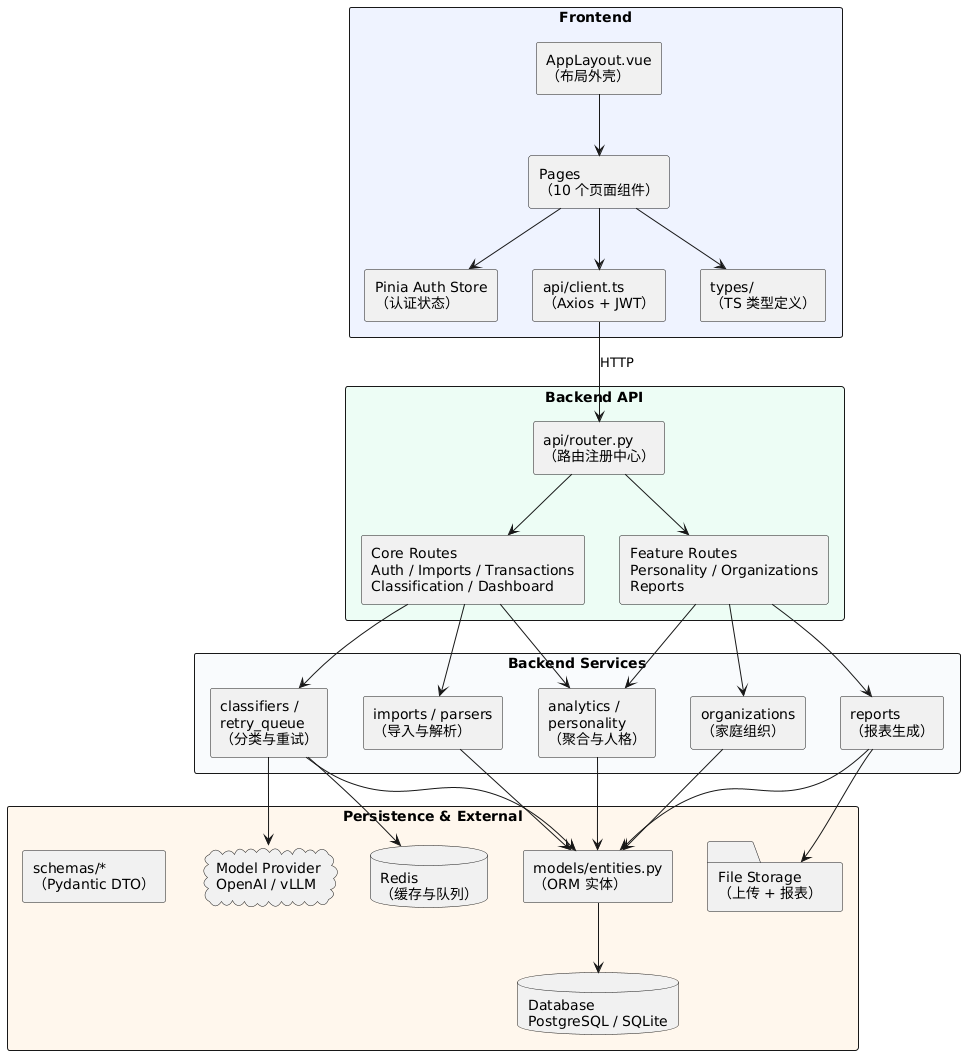
\includegraphics[width=0.92\textwidth]{UML组件图.png}
  \caption{UML 组件图}
  \label{fig:uml-component}
\end{figure}

\begin{figure}[H]
  \centering
  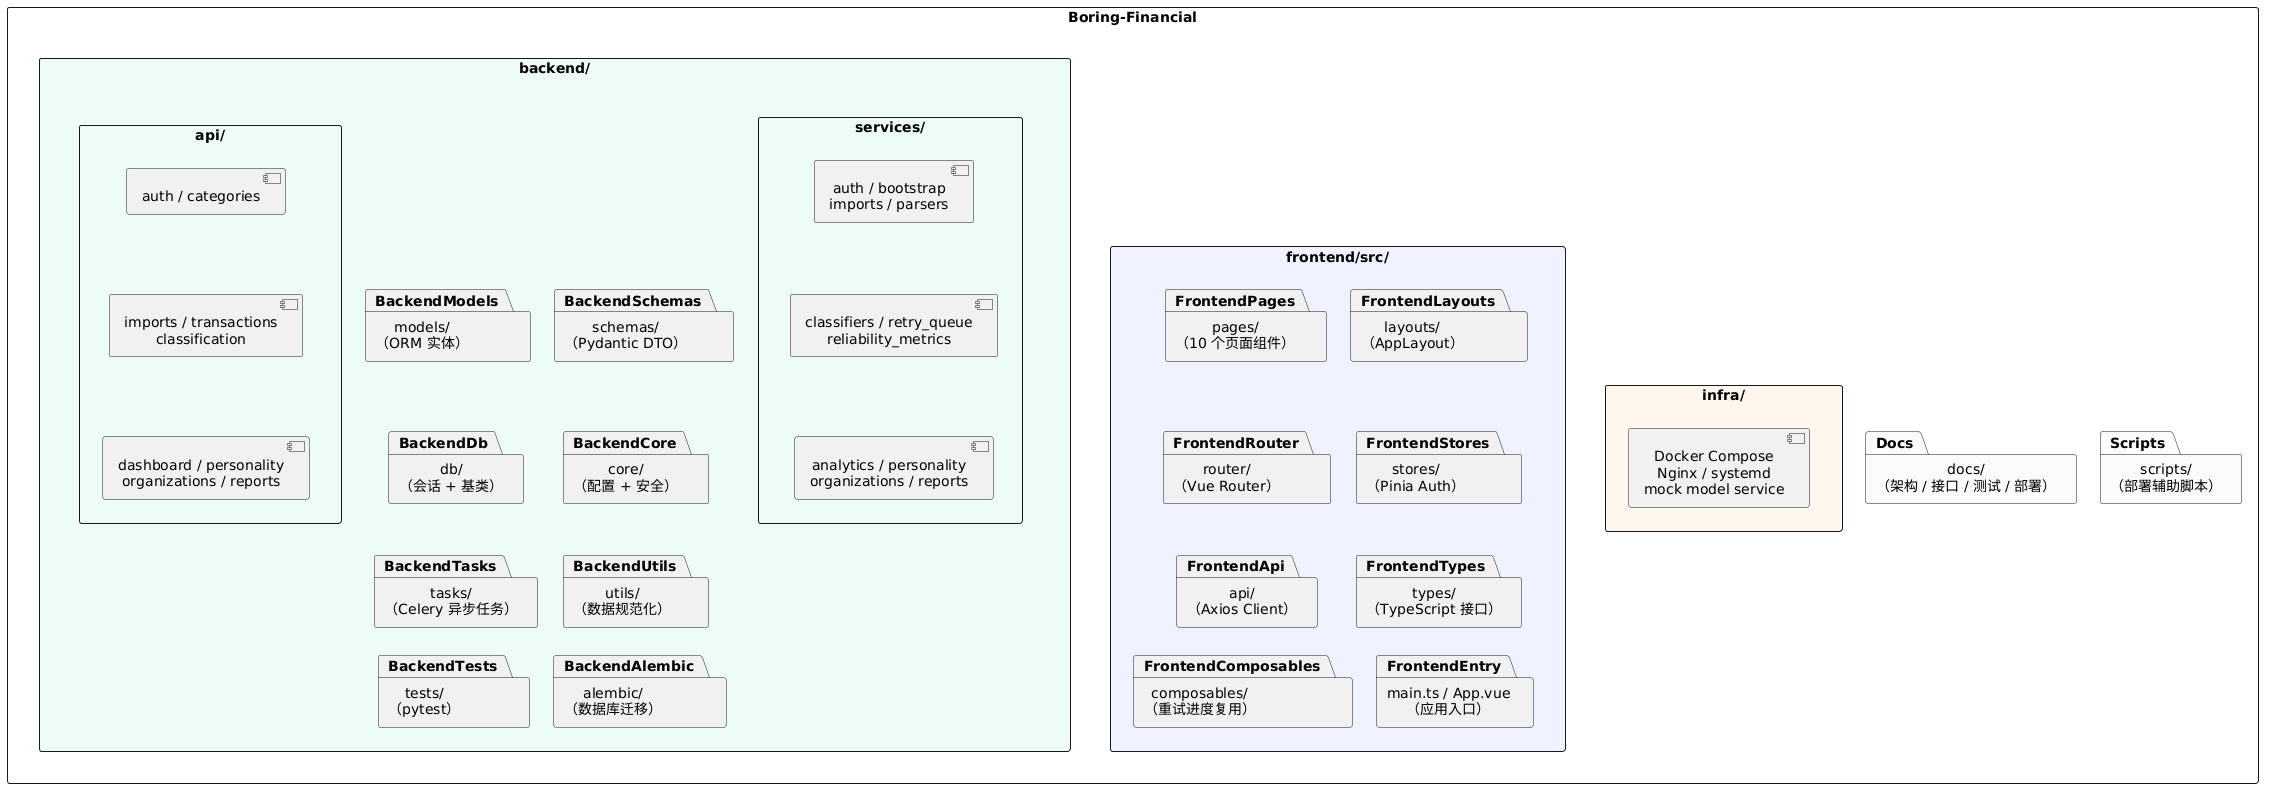
\includegraphics[width=0.92\textwidth]{包图.png}
  \caption{系统包图}
  \label{fig:package}
\end{figure}

\section{后端架构}

后端按分层架构组织为四层。接口层统一接收请求，完成身份校验、输入验证和响应组织；业务层承担导入、解析、分类、财务分析、消费人格、家庭组织和报表生成等业务规则；数据层使用对象关系映射（ORM）描述 12 个领域实体，并负责持久化访问；基础设施层提供数据库会话、安全配置、文件存储和可选的异步任务能力。各层通过明确的数据契约交互，使业务规则不依赖具体的网络协议或数据库实现。

\section{核心模块职责}

\begin{longtable}{p{2.7cm} p{3.5cm} p{4.0cm} p{3.5cm}}
\caption{核心业务模块划分}
\label{tab:core-modules}\\
\toprule
\textbf{模块} & \textbf{划分理由} & \textbf{主要职责} & \textbf{核心数据对象} \\
\midrule
\endfirsthead
\multicolumn{4}{c}{\small 表~\thetable\quad 核心业务模块划分（续）} \\
\toprule
\textbf{模块} & \textbf{划分理由} & \textbf{主要职责} & \textbf{核心数据对象} \\
\midrule
\endhead
\midrule
\multicolumn{4}{r}{\small 接下页} \\
\endfoot
\bottomrule
\endlastfoot
认证与授权 & 身份和资源归属是全部业务操作的共同前置条件 & 注册登录、身份凭证校验、当前用户识别、管理员权限 & 用户、身份凭证 \\
\hline
导入与解析 & 平台文件差异变化频繁，应与下游业务隔离 & 保存文件、维护批次、平台识别、解析、规范化与去重 & 导入批次、上传文件、标准交易 \\
\hline
分类与重试 & 分类服务可能不可用且需要替换，需要统一协调 & 缓存查询、模型与规则分类、分类历史、重试状态与失败恢复 & 分类结果、分类缓存、重试状态 \\
\hline
交易与分类管理 & 交易查询与人工最终分类属于用户控制边界 & 分页筛选、详情、人工校正、系统与自定义分类维护 & 交易、分类 \\
\hline
分析与人格 & 多个页面共享相同交易聚合口径 & 财务指标、趋势、消费人格、问卷偏差与财务健康 & 聚合指标、人格画像 \\
\hline
家庭组织 & 组织权限与个人归属规则独立于普通交易管理 & 组织和成员管理、基于角色的访问控制（RBAC）、成员范围确定 & 组织、组织成员、成员角色 \\
\hline
报表 & PDF 构建包含独立的数据准备和渲染步骤 & 创建任务记录、准备报表数据、生成并下载 PDF & 报表任务、报表文件 \\
\bottomrule
\end{longtable}

图~\ref{fig:billing-data-flow} 将导入、分类、人工校正与后续分析串联为一条数据主线。系统分别保存自动建议和人工确定的最终分类；财务看板、消费人格和报表统一优先使用最终分类，避免不同功能采用不同统计口径。

\begin{figure}[p]
  \centering
  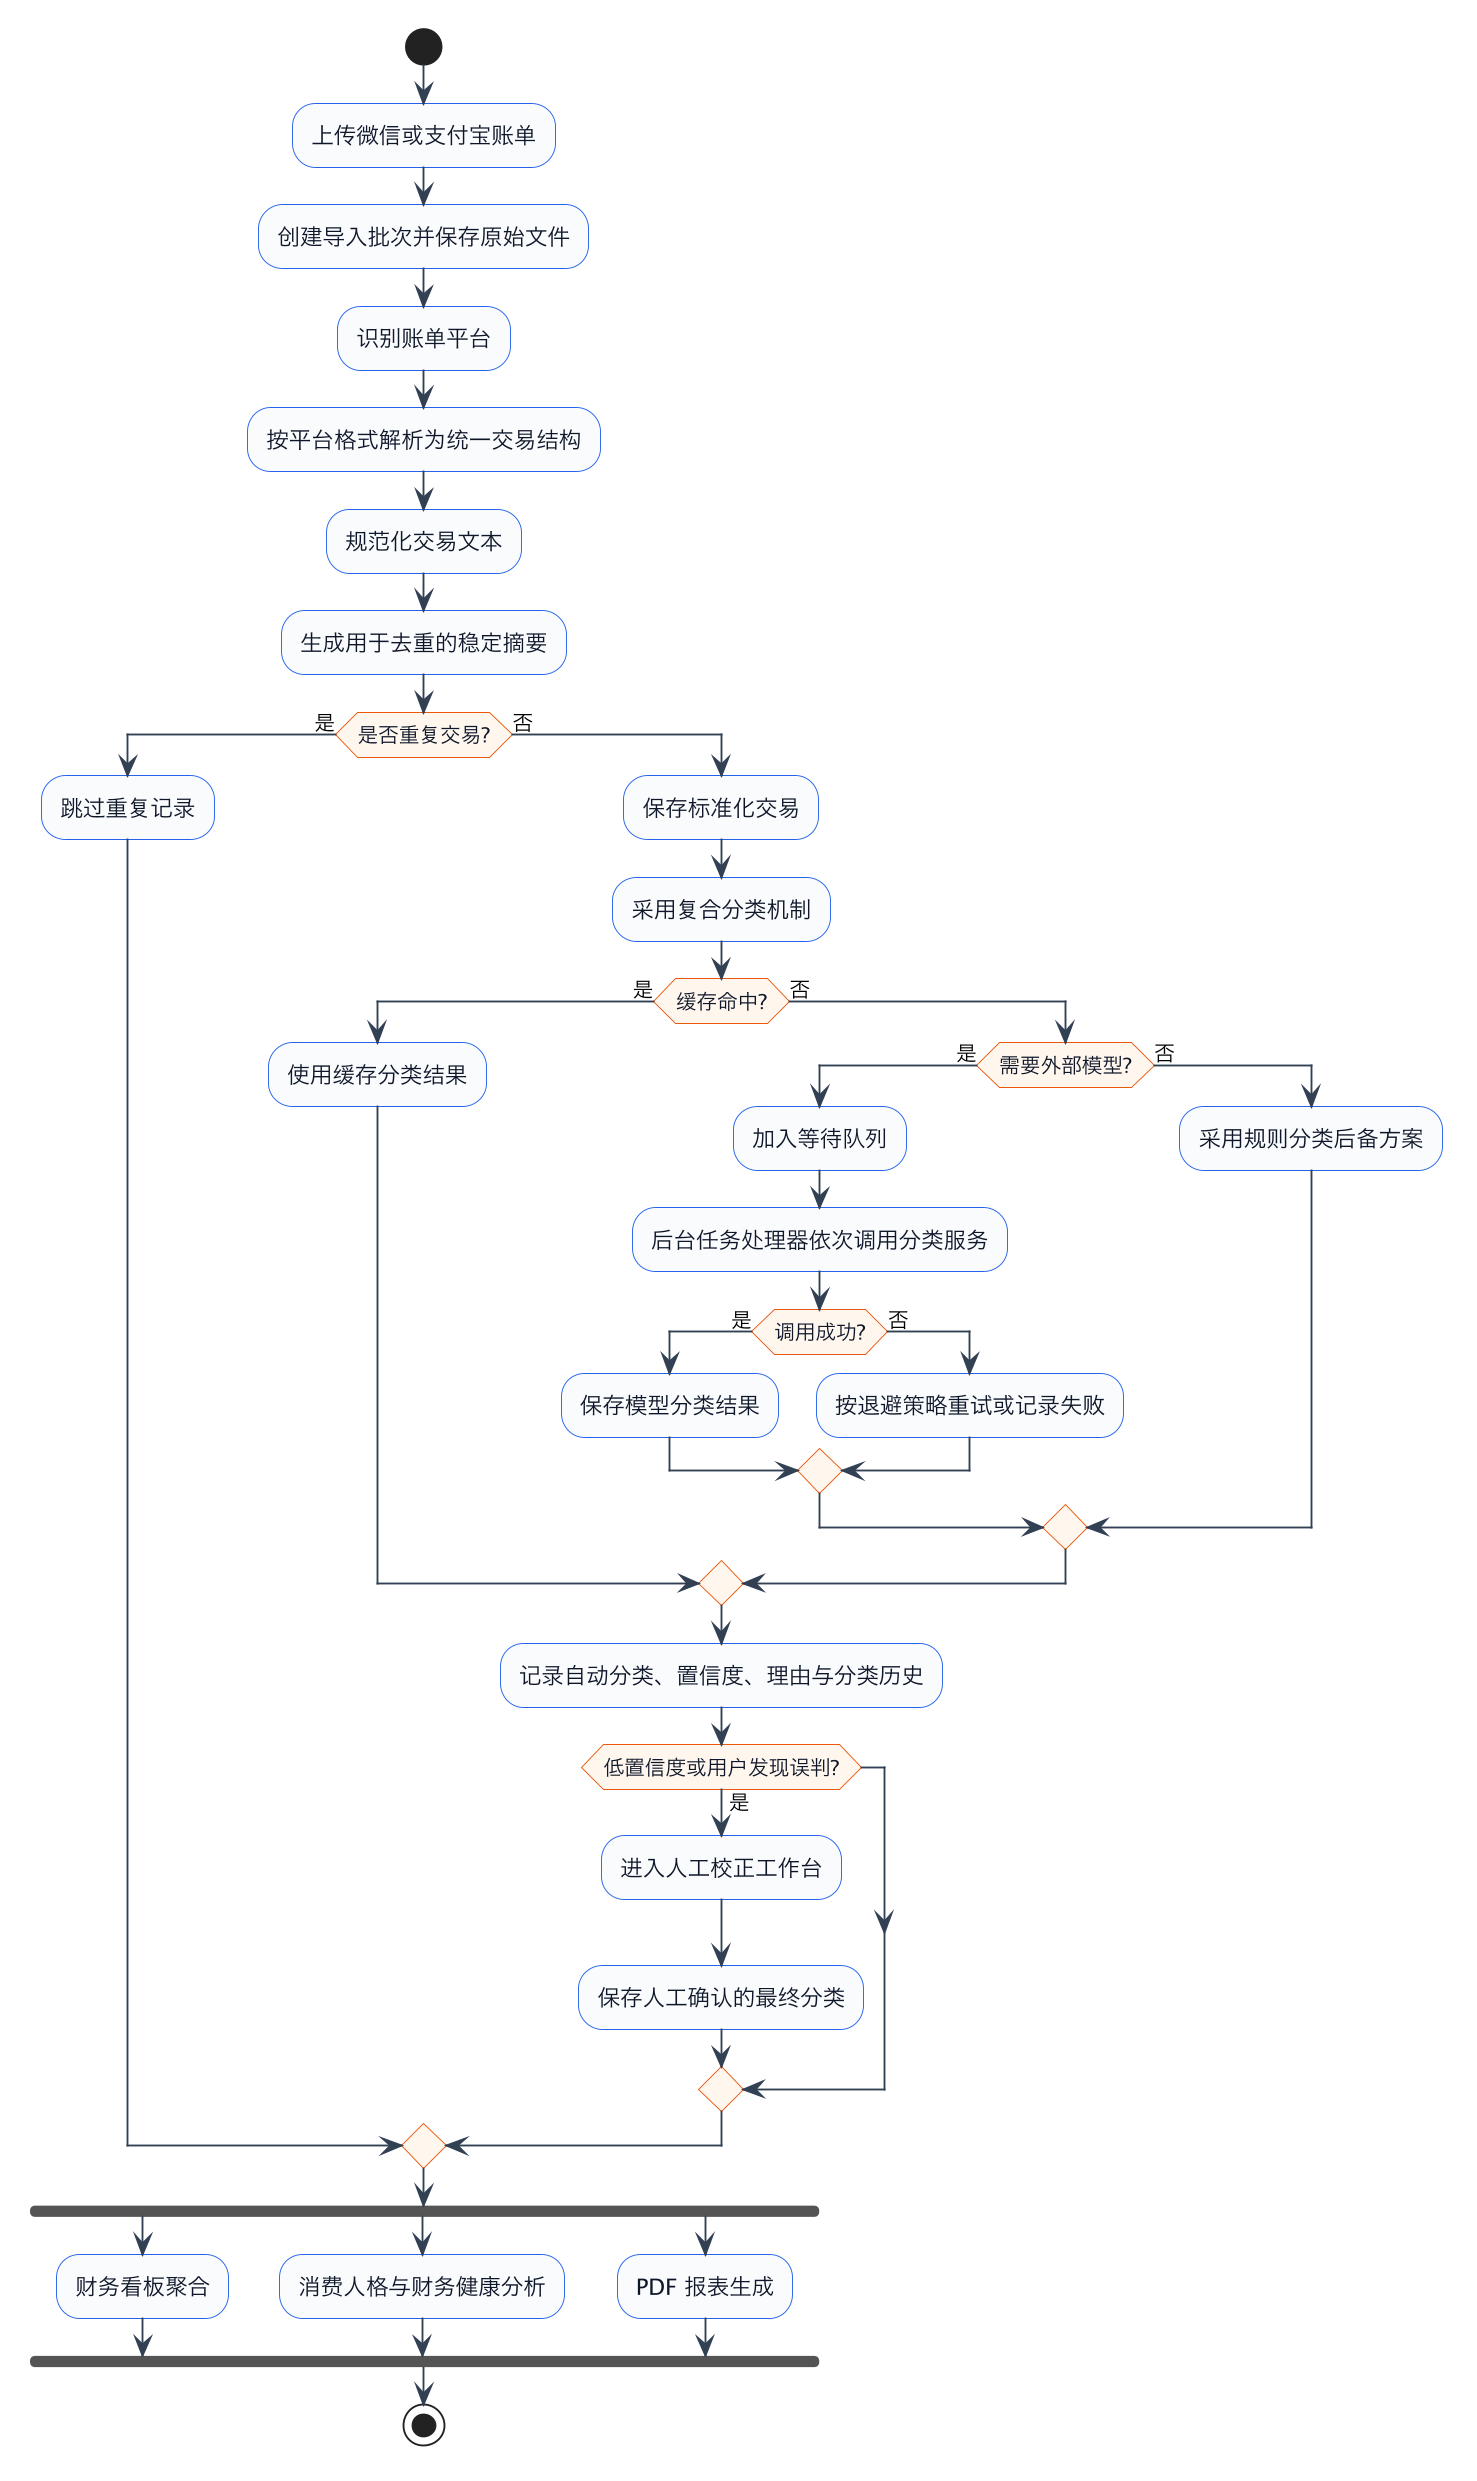
\includegraphics[width=\textwidth,height=0.92\textheight,keepaspectratio]{billing-data-flow.png}
  \caption{账单处理核心数据流图}
  \label{fig:billing-data-flow}
\end{figure}

\section{数据隔离策略}

系统通过以下机制保障多用户数据隔离与家庭组织聚合访问：

\begin{enumerate}
  \item \textbf{个人资源归属}：交易、导入批次、上传文件、分类缓存和报表等私有资源均记录所属用户；系统分类与用户自定义分类采用不同的归属规则。
  \item \textbf{访问范围过滤}：系统根据身份凭证识别当前用户，并在每次私有资源访问时同时校验资源归属，避免仅凭资源编号访问他人数据。
  \item \textbf{家庭聚合模式}：家庭组织不改变交易归属。用户选择家庭视图时，系统先校验组织成员身份，再将可访问范围扩展为组织内成员的数据集合。
  \item \textbf{默认模式}：未选择家庭视图时，各项分析均按个人账本口径返回数据，保持个人功能的独立性。
\end{enumerate}

\section{部署架构}

系统支持两种部署模式以适应不同规模的运行环境：

\begin{description}
  \item[轻量本地部署] 使用 SQLite 作为数据库；导入与重试任务由应用内后台处理器执行，适合开发、演示和低负载环境。
  \item[Docker Compose 部署] PostgreSQL、Redis、FastAPI、前端静态站点、Nginx、独立任务处理器和可选本地模型服务分别运行，适合需要稳定数据服务和任务隔离的环境。
\end{description}

通信过程为：用户浏览器访问 Nginx，静态资源由其直接返回，业务请求转发至 FastAPI，再由应用访问数据库和文件存储。独立任务处理器可通过 Redis 接收异步任务；重试任务处理器从数据库读取等待处理的交易并调用分类服务。上传文件与 PDF 报表统一保存于文件存储区域。

\begin{figure}[H]
  \centering
  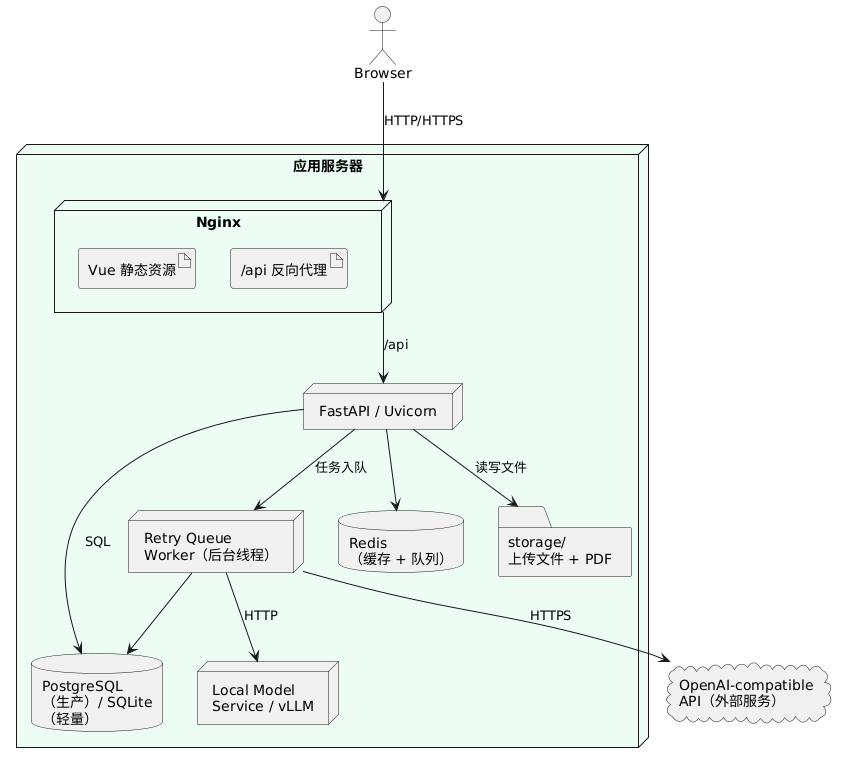
\includegraphics[width=0.92\textwidth]{部署图.png}
  \caption{系统部署图}
  \label{fig:deployment}
\end{figure}

\headingneedspace{28}
\section{安全机制}

系统的安全设计覆盖认证、授权、数据隔离、注入防护与隐私保护五个层面。

认证与授权能力作为接口层的统一前置检查：系统先验证用户身份，再根据业务操作检查资源归属或管理员权限。该设计将安全规则集中管理，使认证策略的变化尽量不影响具体业务逻辑。

\begingroup
\footnotesize
\renewcommand{\arraystretch}{1.18}
\begin{longtable}{@{}p{2.8cm} p{3.8cm} p{3.4cm} p{3.4cm}@{}}
  \caption{安全机制汇总}
  \label{tab:security}\\
    \toprule
    \textbf{安全风险} & \textbf{应对措施} & \textbf{适用层次} & \textbf{说明} \\
    \midrule
    \endfirsthead
    \multicolumn{4}{c}{\small 表~\thetable\quad 安全机制汇总（续）} \\
    \toprule
    \textbf{安全风险} & \textbf{应对措施} & \textbf{适用层次} & \textbf{说明} \\
    \midrule
    \endhead
    \midrule
    \multicolumn{4}{r}{\small 接下页} \\
    \endfoot
    \bottomrule
    \endlastfoot
    身份伪造 & 密码摘要存储与 JSON Web Token（JWT）双凭证机制 & 认证层 & 密码不存明文；访问凭证具有较短有效期 \\
    \hline
    未授权访问 & 受保护操作必须验证用户身份 & 接口层 & 每次请求均校验身份凭证及有效期 \\
    \hline
    跨用户数据泄露 & 私有资源访问同时校验当前用户与资源归属 & 业务层与数据层 & 即使资源编号有效，也不能访问其他用户的数据 \\
    \hline
    组织越权操作 & 基于角色的访问控制 & 组织管理模块 & 所有者可管理成员与角色，普通成员仅可查看授权数据 \\
    \hline
    SQL 注入 & 对象关系映射与参数化查询 & 数据访问层 & 业务查询不直接拼接 SQL 字符串 \\
    \hline
    恶意文件上传 & 清理文件名并仅交由受支持的账单解析器处理 & 导入模块 & 当前尚未实现文件大小、内容类型和扩展名的完整前置校验，列为后续加固项 \\
    \hline
    模型隐私 & 商户名称与商品摘要可能被发送至外部服务 & 分类模块 & 已识别为风险点；可通过本地模型选项减少外部传输 \\
\end{longtable}
\endgroup

\chapter{程序开发}

本章从程序结构角度说明领域实体、分类策略、账单解析和报表生成的设计，并进一步介绍数据库、模块间数据契约、设计模式及核心业务流程。重点在于说明设计职责和协作关系，而非逐项解释源代码。

\section{面向对象程序组织}

系统根据问题特征选择程序组织方式：领域对象、可替换分类策略、平台解析器和报表构建过程采用面向对象设计；身份校验、数据聚合等流程则以分层服务组织。二者共同服务于职责分离、扩展性和可测试性。

\subsection{领域实体及其关联关系}

系统使用对象关系映射（ORM）描述 12 个领域实体，并采用数据映射模式将领域结构与数据库访问分离。实体关系围绕五个业务域展开：用户拥有个人交易与自定义分类；导入批次包含一个或多个上传文件，并产生标准化交易；交易保留自动分类建议、人工最终分类和历次分类记录；家庭组织通过成员关系连接多个用户；报表任务记录生成过程并关联最终文件。

交易去重依据发生时间、金额、商户、商品和备注等规范化信息生成稳定摘要，并由数据库唯一约束阻止同一用户重复保存相同交易。分类设计同时保留“自动建议”和“人工最终决定”，各项分析优先采用人工确认结果。分类历史采用追加方式保存，使分类来源和结果变化可以追溯。图~\ref{fig:entity-class} 仅列出参与领域关系的关键属性，其他实现字段由数据库设计图补充。

\begin{figure}[p]
  \centering
  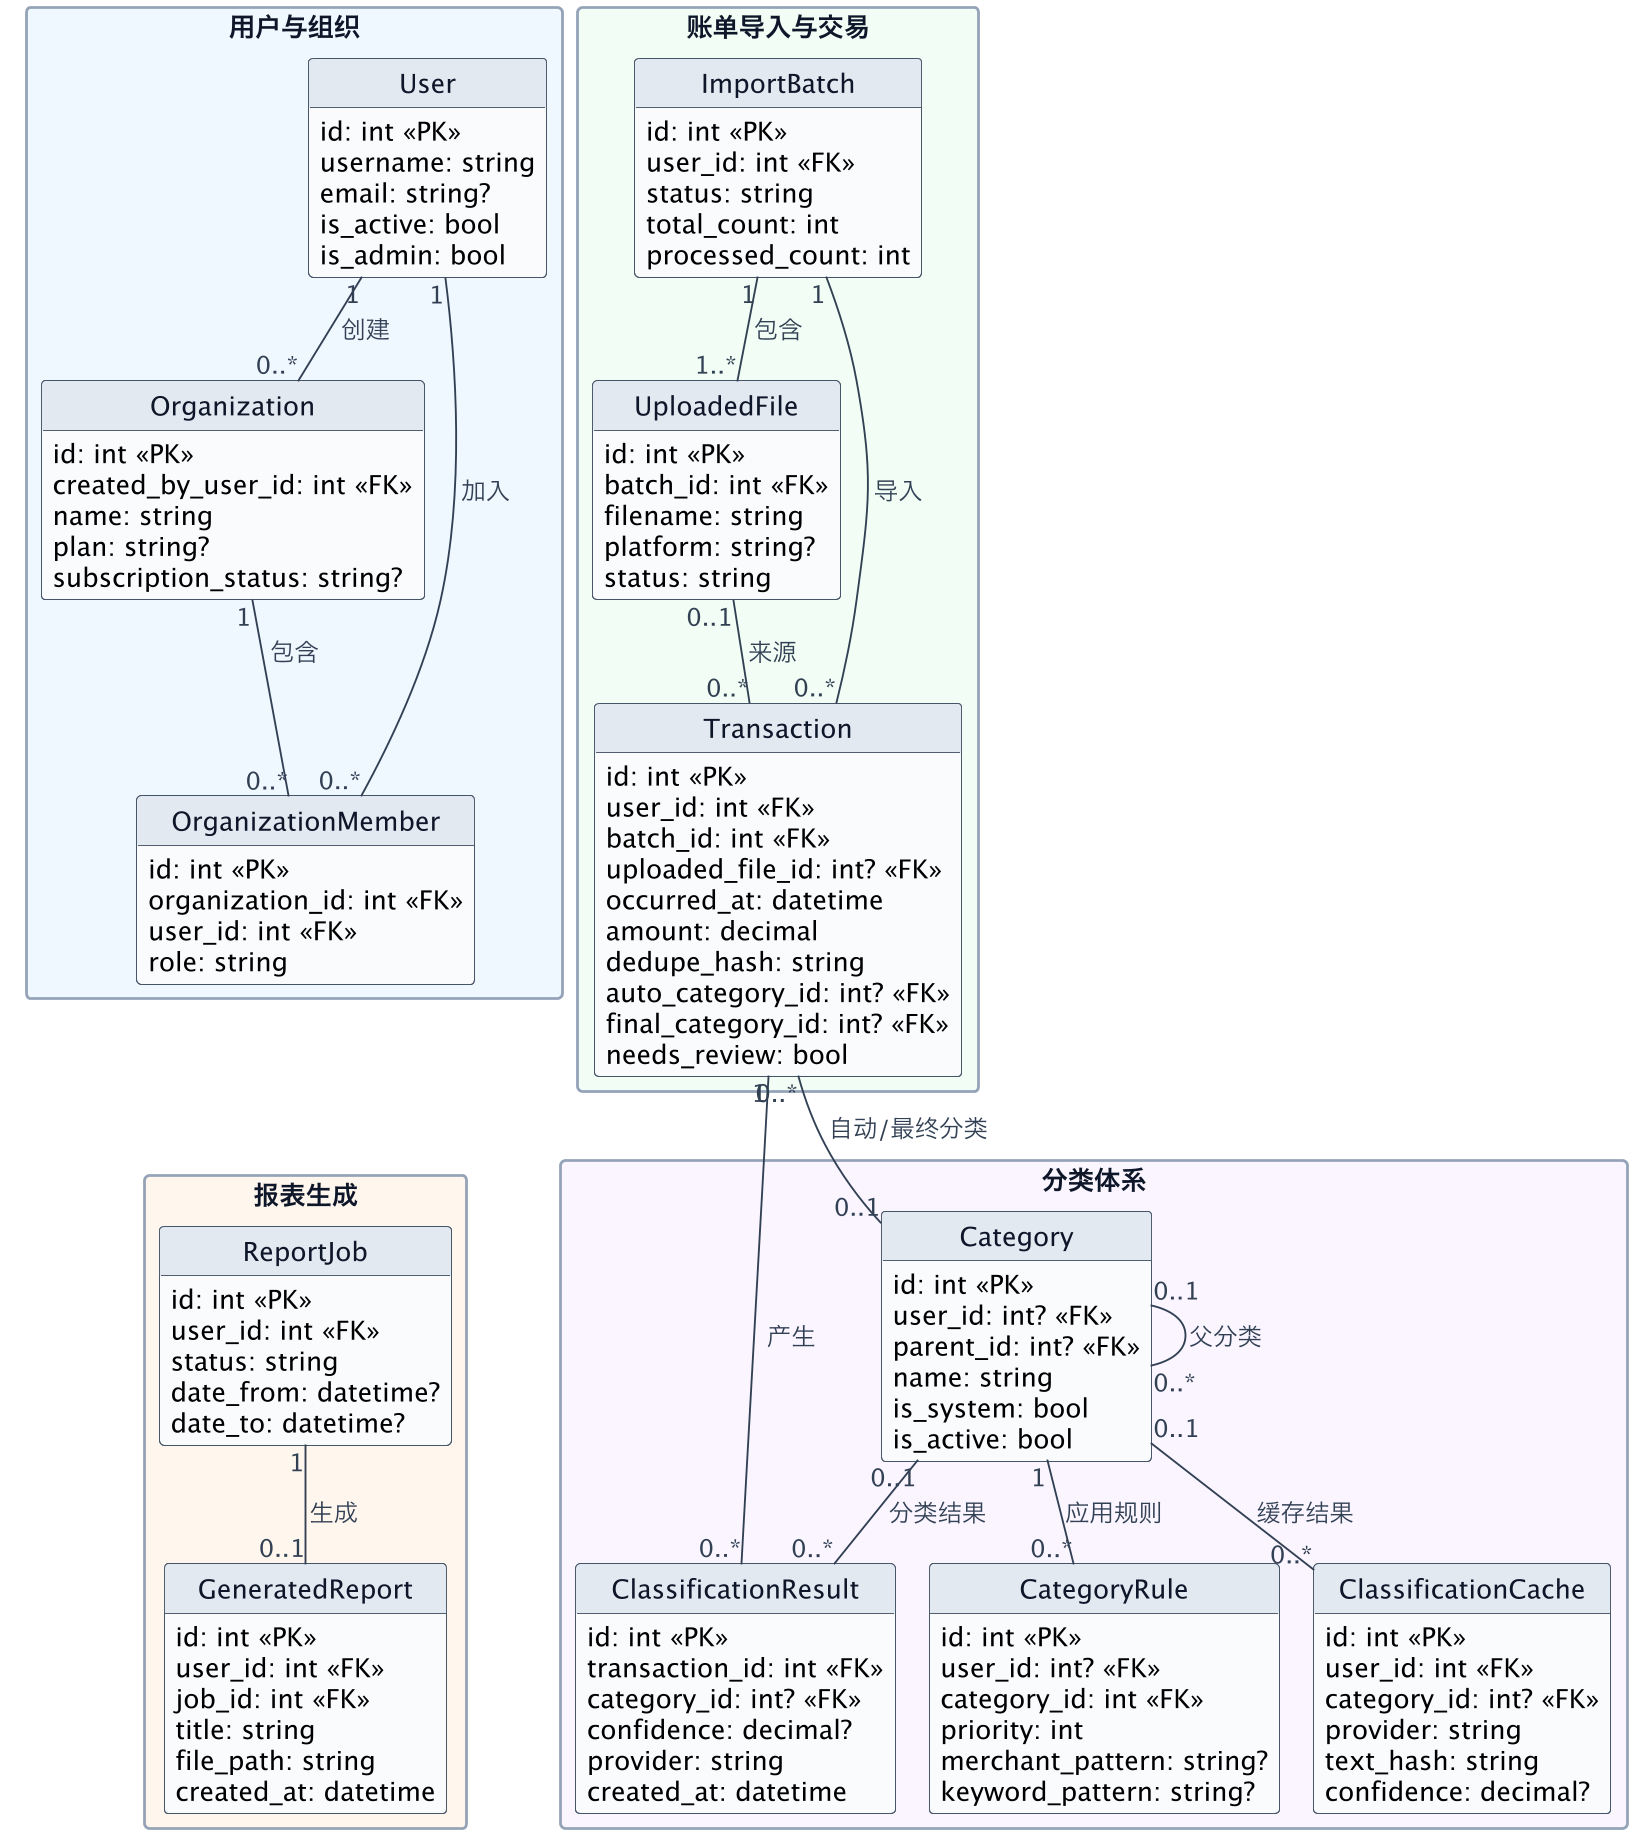
\includegraphics[
    width=0.92\textwidth,
    height=0.76\textheight,
    keepaspectratio
  ]{entity-domain-model.png}
  \caption{领域实体类图}
  \label{fig:entity-class}
\end{figure}

\subsection{分类器策略}

分类子系统采用策略、责任链和外观三种模式。缓存分类、模型分类和规则分类遵循统一的数据契约，可以根据运行配置替换；分类请求依次尝试已有缓存、模型服务和规则后备方案，在外部服务不可用时仍能给出可解释结果；统一入口负责协调缓存、模型调用、失败重试和结果保存，使导入模块不需要了解各类分类方式的内部差异。

外部模型调用由等待队列控制，并采用指数退避减少持续失败时的请求压力。无论结果来自缓存、外部模型、本地模型还是规则，系统都统一记录类别、置信度、理由和来源，便于后续展示、人工校正和质量分析。分类器之间的静态关系如图~\ref{fig:classifier-class} 所示。

\begin{figure}[!htbp]
  \centering
  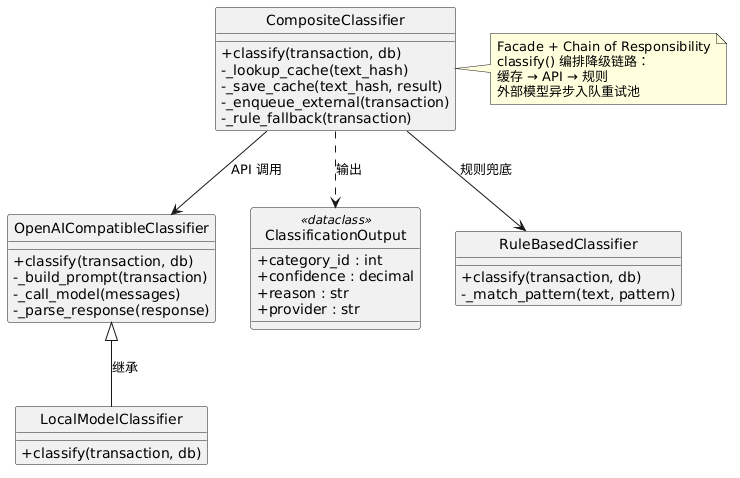
\includegraphics[
    width=0.66\textwidth,
    height=0.30\textheight,
    keepaspectratio
  ]{分类器策略类图.png}
  \caption{分类器策略类图}
  \label{fig:classifier-class}
\end{figure}

\subsection{账单解析器}

解析子系统负责将微信和支付宝的异构账单转换为统一交易结构，采用策略、适配器与注册表思想。系统首先根据文件名和内容特征识别平台，再处理不同编码、文件格式和表头位置，最后将平台特有列名映射为统一的时间、金额、商户、商品和状态等信息。规范化阶段统一字符形式并生成去重摘要。

不同平台的解析规则彼此独立，新平台只需提供识别规则和字段映射，不需要修改分类、分析和报表模块。统一读取能力屏蔽 CSV 与 Excel、字符编码和表头位置等差异；注册机制负责选择合适的平台解析策略。该结构降低了新增账单来源对其他模块的影响，类之间的关系如图~\ref{fig:parser-class} 所示。

\begin{figure}[H]
  \centering
  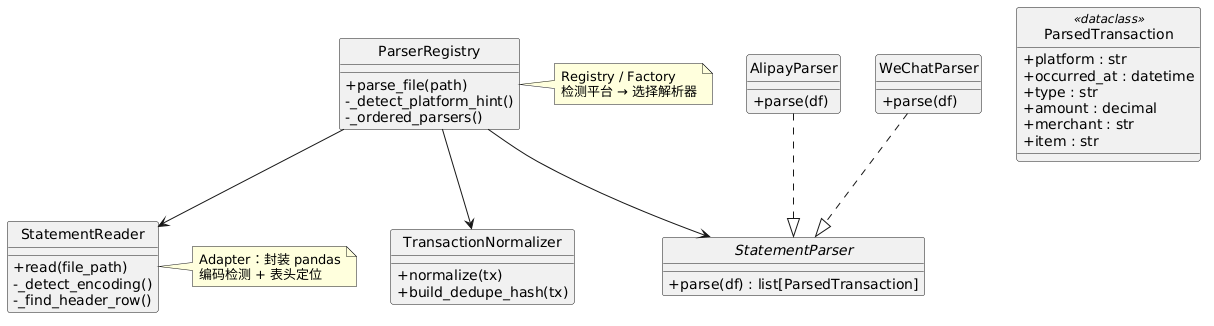
\includegraphics[width=0.92\textwidth]{解析器类图.png}
  \caption{账单解析器类图}
  \label{fig:parser-class}
\end{figure}

\subsection{报表构建器}

报表子系统采用构建器模式，将数据准备、封面生成、摘要指标、分类汇总、商户排行和交易明细等步骤有序组合。数据聚合与页面渲染相互分离，同一份报表数据可以被多个页面区域复用；各渲染步骤职责单一，增加新章节时只需扩展构建过程，而不必修改已有统计逻辑。

系统同时考虑中文字体兼容和输出文件记录，使报表在不同运行环境下保持可读，并能够通过任务记录追踪生成结果。报表构建器的结构如图~\ref{fig:reportbuilder-class} 所示。

\begin{figure}[H]
  \centering
  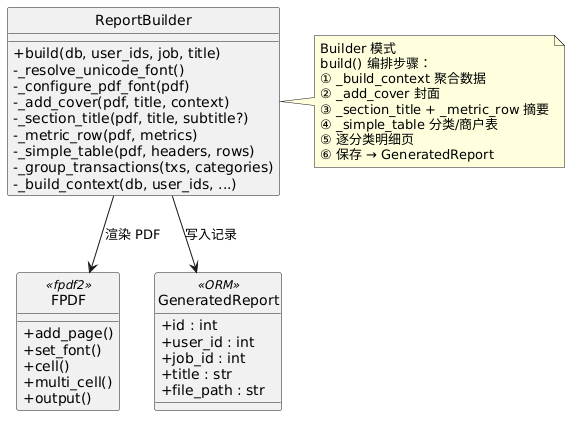
\includegraphics[width=0.85\textwidth]{报表构建器类图.png}
  \caption{报表构建器类图}
  \label{fig:reportbuilder-class}
\end{figure}

\section{数据库设计}

系统数据库共 12 张表，按业务域分两组展示。

\subsection{核心账单与分类}

核心域由用户、分类、分类规则、导入批次、上传文件、交易、分类历史和分类缓存八类数据组成。

\begin{figure}[H]
  \centering
  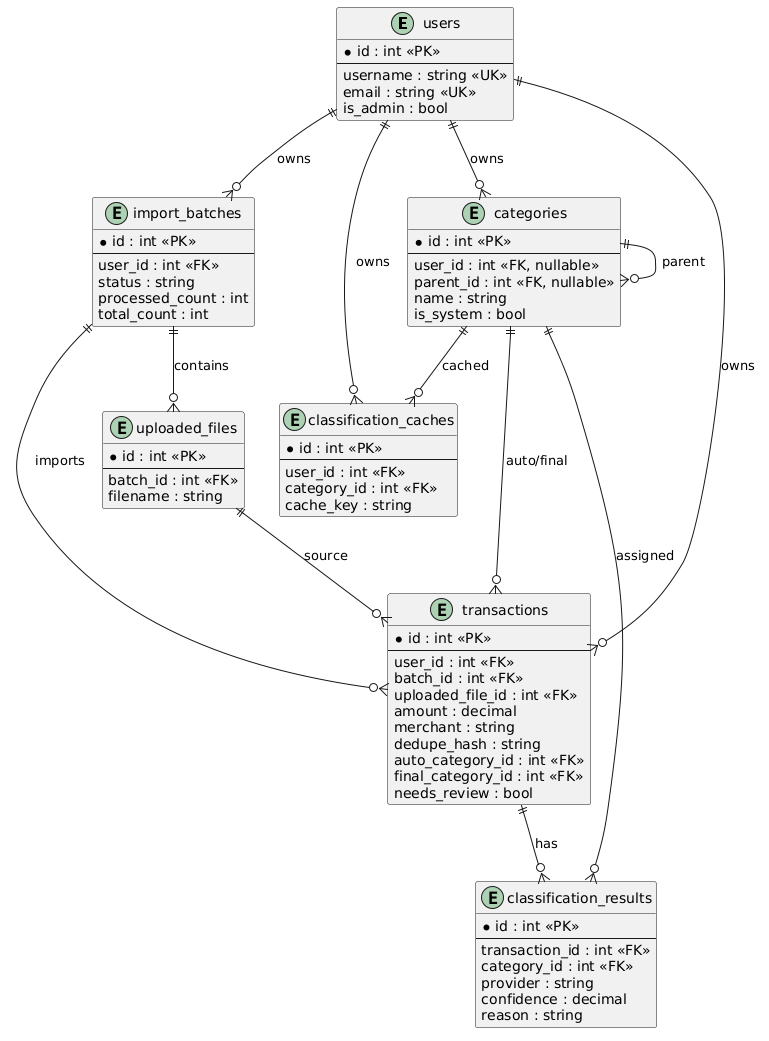
\includegraphics[
    width=0.60\textwidth,
    height=0.56\textheight,
    keepaspectratio
  ]{核心账单ER图.png}
  \caption{核心账单与分类 ER 图}
  \label{fig:er-core}
\end{figure}

关键设计决策包括：以用户和交易摘要的联合唯一约束阻止重复导入；分别保存自动分类建议与人工最终分类，并优先采用人工结果；以复核标记识别低置信度或未分类交易；分类历史只追加不覆盖，以保留每次分类记录；分类缓存按用户、分类服务和文本摘要隔离，避免不同用户之间共享敏感结果。

\subsection{家庭组织与报表扩展}

扩展域由家庭组织、组织成员、报表任务和生成报表四类数据组成，并与用户和交易数据共享关联。

组织成员角色分为所有者、管理员和普通成员：所有者拥有完整管理权限，管理员可管理普通成员，普通成员仅可查看授权的聚合数据。家庭组织不改变交易的个人归属，家庭分析在查询时依据成员关系扩展数据范围。报表任务记录生成请求的处理阶段，生成报表记录最终文件及其所属用户。

\begin{figure}[H]
  \centering
  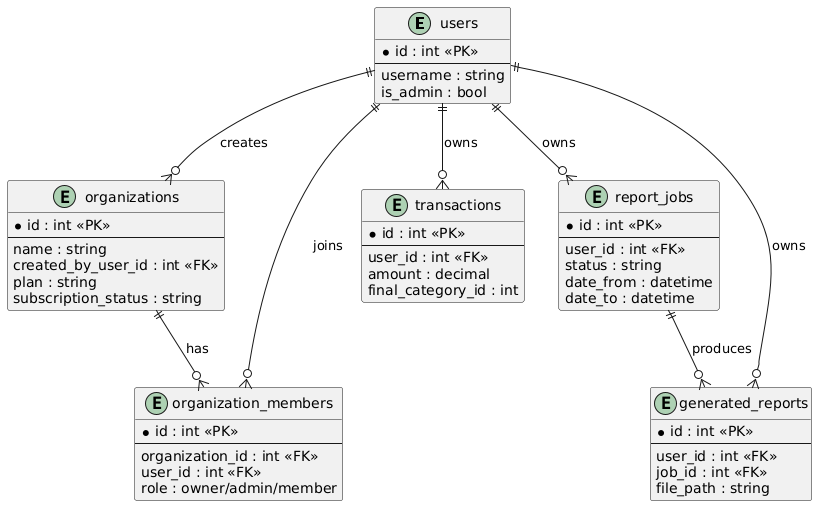
\includegraphics[width=0.92\textwidth]{家庭组织与报表扩展ER图.png}
  \caption{家庭组织与报表扩展 ER 图}
  \label{fig:er-family}
\end{figure}

\section{接口设计}

\subsection{外部 REST API}

系统对外接口采用统一前缀管理，除注册、登录与健康检查外均要求身份凭证。表~\ref{tab:api-overview} 集中列出主要接口及访问权限；更详细的请求与响应结构由 OpenAPI 接口文档描述。

\begingroup
\footnotesize
\setlength{\tabcolsep}{3pt}
\begin{longtable}{@{}p{2.3cm} p{3.2cm} p{2.5cm} p{2.1cm} p{2.2cm}@{}}
\caption{主要外部 API 接口}
\label{tab:api-overview}\\
\toprule
\textbf{方法} & \textbf{路径} & \textbf{功能} & \textbf{权限} & \textbf{关键输入/输出} \\
\midrule
\endfirsthead
\multicolumn{5}{c}{\small 表~\thetable\quad 主要外部 API 接口（续）} \\
\toprule
\textbf{方法} & \textbf{路径} & \textbf{功能} & \textbf{权限} & \textbf{关键输入/输出} \\
\midrule
\endhead
\midrule
\multicolumn{5}{r}{\small 接下页} \\
\endfoot
\bottomrule
\endlastfoot
POST & \path{/api/auth/register}、\path{/login} & 注册或登录并返回身份凭证 & 无 & 用户名、密码、用户信息与身份凭证 \\
\hline
GET & \path{/api/auth/me} & 获取当前用户 & 登录用户 & 当前用户信息 \\
\hline
\shortstack[l]{GET/POST/\\PATCH} & \path{/api/categories} & 查询、创建和更新分类 & 登录用户 & 分类信息 \\
\hline
POST & \path{/api/imports} & 上传一个或多个账单文件 & 登录用户 & 文件与导入批次信息 \\
\hline
\shortstack[l]{GET/\\DELETE} & \path{/api/imports[/{batch_id}]} & 查询批次、文件或删除本人批次 & 资源所有者 & 批次状态、进度、错误信息 \\
\hline
GET & \path{/api/transactions} & 分页筛选交易 & 登录用户 & 日期、平台、分类、文件、关键词 \\
\hline
PATCH & \path{/api/transactions/{id}/category} & 确认或修改最终分类 & 资源所有者 & \texttt{category\_id}、\texttt{mark\_reviewed} \\
\hline
POST & \path{/api/classification/reclassify} & 对本人指定交易重新分类 & 登录用户 & 交易编号列表、分类服务 \\
\hline
\shortstack[l]{GET/\\POST} & \path{/api/classification/retry-status}、\path{/retry-all} & 查询重试状态或恢复失败交易 & 系统管理员 & 聚合状态或恢复数量 \\
\hline
GET & \path{/api/dashboard/summary} & 获取个人或家庭聚合分析 & 登录用户/组织成员 & 日期、文件、组织编号 \\
\hline
\shortstack[l]{GET/\\POST} & \path{/api/personality/profile}、\path{/quiz/result} & 获取画像或提交问卷 & 登录用户/组织成员 & 画像、健康评分、偏差分析 \\
\hline
\shortstack[l]{GET/POST\\PATCH/DELETE} & \path{/api/organizations} & 组织与成员管理 & 登录用户；写操作按角色 & 组织、成员和角色信息 \\
\hline
\shortstack[l]{POST/\\GET} & \path{/api/reports}、\path{/reports/{id}/download} & 生成或下载 PDF 报表 & 登录用户/组织成员、所有者 & 日期、文件、报表文件 \\
\hline
\shortstack[l]{GET/\\PUT} & \path{/api/settings} & 查询或保存用户分类设置 & 登录用户 & 分类服务、模型名、置信度阈值 \\
\hline
GET & \path{/health} & 应用存活探测 & 无 & 服务状态 \\
\end{longtable}
\endgroup

接口错误遵循 HTTP 状态码语义：未提供有效凭据返回 401，组织角色不足返回 403，资源不存在或不属于当前用户时通常返回 404，请求字段不符合 Pydantic 模型时返回 422，解析或文件生成等内部异常返回 500。资源归属场景使用 404 可以避免向调用者泄露目标资源是否存在。

\subsection{模块间数据契约}

\begin{table}[H]
\centering
\small
\caption{模块间数据契约}
\label{tab:internal-contracts}
\begin{tabularx}{0.98\textwidth}{p{3.3cm} p{4.2cm} X}
\toprule
\textbf{协作边界} & \textbf{输入与输出} & \textbf{作用} \\
\midrule
账单解析 & 原始账单文件 $\rightarrow$ 平台信息与标准交易列表 & 隔离微信、支付宝等原始列名差异，后续模块只使用统一交易结构。 \\
\hline
智能分类 & 标准交易 $\rightarrow$ 分类结果 & 协调缓存、模型、规则后备方案和失败重试，调用方不依赖具体分类方式。 \\
\hline
分类结果 & 类别、子类别、置信度、理由、来源 & 统一规则、外部服务和本地模型的输出格式，便于保存与展示。 \\
\hline
家庭成员范围 & 组织编号 $\rightarrow$ 可访问成员范围 & 将家庭权限校验与财务分析、消费人格、报表聚合相互分离。 \\
\hline
报表生成 & 用户范围、日期和文件筛选 $\rightarrow$ PDF 报表 & 将报表数据准备、页面渲染和结果记录组织为统一过程。 \\
\hline
接口数据模型 & JSON 或表单输入 $\leftrightarrow$ 数据传输对象 & 在 HTTP 边界执行字段校验和序列化，避免直接暴露数据库实体。 \\
\bottomrule
\end{tabularx}
\end{table}

\subsection{任务与状态语义}

\begin{table}[H]
\centering
\small
\caption{任务状态与故障语义}
\label{tab:task-status}
\begin{tabularx}{0.98\textwidth}{p{3cm} p{4.2cm} X}
\toprule
\textbf{任务} & \textbf{状态或流转} & \textbf{说明} \\
\midrule
账单导入 & 等待处理 $\rightarrow$ 处理中 $\rightarrow$ 完成/部分失败/失败 & 后台处理过程更新总数与已处理数；部分记录失败时保留成功数据并记录原因。 \\
\hline
外部模型分类 & 等待重试 $\rightarrow$ 分类完成/重试失败 & 后台任务处理器依次处理等待交易，并记录最终分类来源或失败结果。 \\
\hline
报表生成 & 当前实现：处理中 $\rightarrow$ 完成 & 当前采用同步方式构建 PDF；系统已经预留等待和失败状态，但异步提交、状态查询和失败反馈尚未形成完整流程。 \\
\bottomrule
\end{tabularx}
\end{table}

\section{设计模式应用}

下表不只列出模式名称，还说明它解决的变化点以及支撑的质量要求。

\begingroup
\footnotesize
\setlength{\tabcolsep}{3pt}
\begin{longtable}{@{}p{2.4cm} p{4.2cm} p{3.4cm} p{2.0cm}@{}}
    \caption{设计模式应用汇总}
    \label{tab:design-patterns}\\
    \toprule
    \textbf{设计模式} & \textbf{解决的问题} & \textbf{主要应用} & \textbf{支撑属性} \\
    \midrule
    \endfirsthead
    \multicolumn{4}{c}{\footnotesize 表~\thetable\quad 设计模式应用汇总（续）} \\
    \toprule
    \textbf{设计模式} & \textbf{解决的问题} & \textbf{主要应用} & \textbf{支撑属性} \\
    \midrule
    \endhead
    \midrule
    \multicolumn{4}{r}{\footnotesize 接下页} \\
    \endfoot
    \bottomrule
    \endlastfoot
    Data Mapper & 将领域实体与具体数据库查询分离，减少持久化方式对业务结构的影响 & 领域实体与数据访问 & 可维护性 \\
    \hline
    Strategy & 在统一协作方式下替换规则、外部模型或本地模型分类，也可替换不同平台解析规则 & 分类与账单解析 & 可扩展性 \\
    \hline
    Chain of Responsibility & 依次尝试缓存、模型和规则，在前一环节不可用时继续处理 & 复合分类过程 & 可靠性 \\
    \hline
    Facade & 对导入模块隐藏缓存、模型调用、失败重试与结果记录的复杂性 & 分类统一入口 & 可维护性 \\
    \hline
    Adapter/Factory & 将不同文件格式和平台字段转换为统一交易结构，并自动选择合适的解析策略 & 账单读取与平台识别 & 兼容性、可扩展性 \\
    \hline
    Builder & 将数据准备、摘要、图表和明细等报表步骤按序组合 & PDF 报表生成 & 可维护性 \\
    \hline
    Producer-Consumer & 将产生分类任务的业务过程与执行外部模型调用的后台过程分离 & 外部模型失败重试 & 可靠性 \\
\end{longtable}
\endgroup

\section{核心流程设计}

\subsection{账单导入与大模型初分}

用户上传账单后的处理过程包含六个阶段。(1) 系统接收文件、创建导入批次并向用户反馈进度；(2) 识别账单平台，将原始列转换为统一交易结构；(3) 规范化文本并依据交易特征执行去重；(4) 按“缓存、模型服务、规则后备方案”的顺序获取分类结果，外部服务失败时由后台重试机制继续处理；(5) 同时保存当前分类结果与可追溯的分类历史，低置信度交易进入人工复核；(6) 汇总成功与失败记录，形成完成、部分失败或失败的批次结果。

\begin{figure}[H]
  \centering
  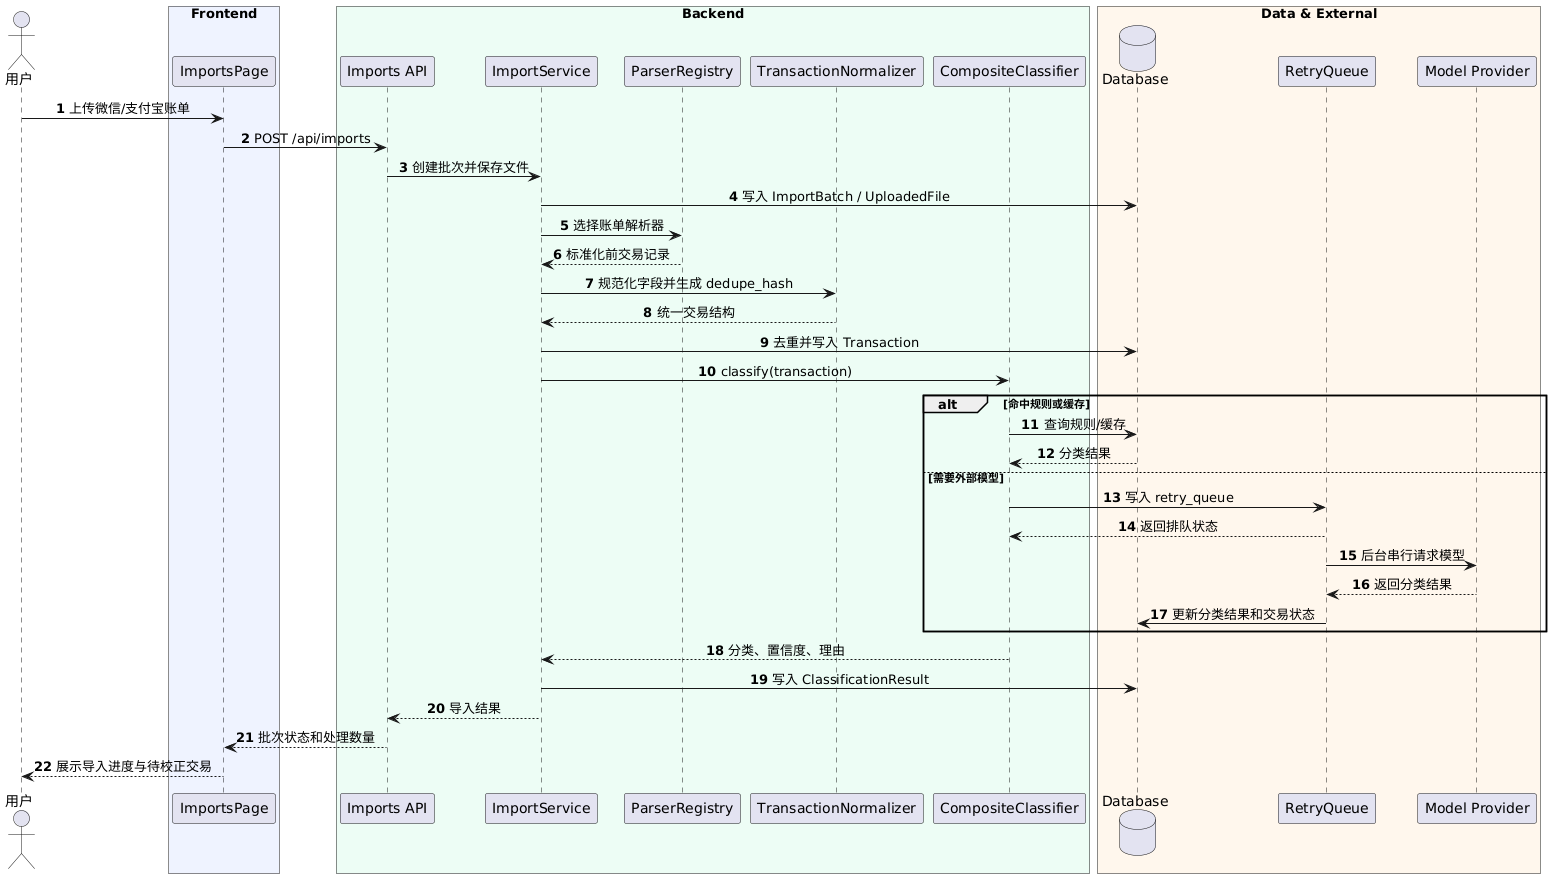
\includegraphics[width=0.92\textwidth]{账单导入与大模型初分顺序图.png}
  \caption{账单导入与大模型初分顺序图}
  \label{fig:seq-import}
\end{figure}

\subsection{家庭组织聚合查询}

家庭组织视图的数据聚合不改变交易的个人归属，而是在查询阶段根据成员身份扩展可访问范围。系统首先取得用户所在组织及其角色；当用户选择家庭财务看板、消费人格或报表时，系统校验成员身份并汇总组织内成员的交易数据。财务看板返回家庭收入、支出、净流入与分类分布，消费人格模块计算家庭整体画像与财务健康评分，报表模块据此生成家庭聚合 PDF。

\begin{figure}[!htbp]
  \centering
  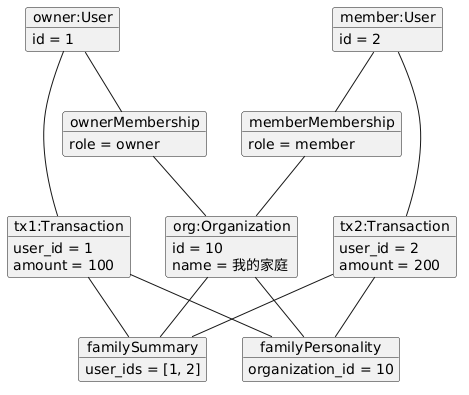
\includegraphics[
    width=0.58\textwidth,
    height=0.32\textheight,
    keepaspectratio
  ]{对象图.png}
  \caption{家庭聚合场景对象图}
  \label{fig:obj-family}
\end{figure}

\chapter{验收与发布}

\section{自动化测试}

\subsection{静态代码验证}

在动态测试之前，团队采用了两类静态验证手段。

\textbf{TypeScript 类型检查}：前端生产构建将静态类型检查作为必要前置步骤，任何类型不兼容错误均会阻断构建。该检查覆盖页面组件、状态管理、通信封装和数据类型定义，用于验证前端数据结构与后端接口契约的一致性。

\textbf{代码走查}：每个开发迭代完成后，团队成员对新增实现进行交叉检查，重点核查身份认证、资源归属、多用户数据隔离和分类异常处理，发现的问题在当前迭代内修正。

\subsection{动态测试}

系统后端建立了覆盖认证、导入、交易、分类、解析、分析、人格、组织、报表和故障重试等领域的自动化测试体系。表~\ref{tab:test-files} 按功能域汇总测试内容与数量，避免以源文件清单代替测试说明。

\begin{longtable}{p{4.2cm} p{7.2cm} p{2.1cm}}
\caption{自动化测试覆盖范围}
\label{tab:test-files}\\
\toprule
\textbf{功能域} & \textbf{主要验证内容} & \textbf{测试数} \\
\midrule
\endfirsthead
\multicolumn{3}{c}{\small 表~\thetable\quad 自动化测试覆盖范围（续）} \\
\toprule
\textbf{功能域} & \textbf{主要验证内容} & \textbf{测试数} \\
\midrule
\endhead
\midrule
\multicolumn{3}{r}{\small 接下页} \\
\endfoot
\bottomrule
\endlastfoot
认证与数据隔离 & 密码摘要、身份凭证、登录流程和受保护资源访问 & 5 \\
\hline
导入、解析与去重 & 多平台账单识别、文本规范化、重复交易识别、批次进度和部分失败处理 & 10 \\
\hline
分类与故障重试 & 提示信息、分类缓存、规则降级、超时重试、失败恢复和可靠性指标 & 14 \\
\hline
交易与报表 & 交易筛选、分页、人工分类、跨用户保护、报表生成与下载 & 7 \\
\hline
数据分析与消费人格 & 财务聚合、日期与分类筛选、人格维度、问卷偏差及边界条件 & 10 \\
\hline
家庭组织 & 组织创建、成员权限、家庭聚合、角色区分和个人模式兼容 & 13 \\
\end{longtable}

\section{需求—设计—测试追踪}

表~\ref{tab:fr-traceability} 和表~\ref{tab:nfr-traceability} 将需求与设计模块、测试证据对应起来。“自动化通过”表示存在可重复执行的测试；“手工验收”表示通过第 7.4 节的用户流程检查；“设计目标”表示尚未完成专项测量，不能解释为已经达到。

\begingroup
\footnotesize
\setlength{\tabcolsep}{3pt}
\begin{longtable}{@{}p{1.0cm} p{2.8cm} p{3.8cm} p{3.6cm} p{1.3cm}@{}}
\caption{功能需求追踪矩阵}
\label{tab:fr-traceability}\\
\toprule
\textbf{ID} & \textbf{设计/实现} & \textbf{测试证据} & \textbf{验收场景} & \textbf{状态} \\
\midrule
\endfirsthead
\multicolumn{5}{c}{\small 表~\thetable\quad 功能需求追踪矩阵（续）} \\
\toprule
\textbf{ID} & \textbf{设计/实现} & \textbf{测试证据} & \textbf{验收场景} & \textbf{状态} \\
\midrule
\endhead
\midrule
\multicolumn{5}{r}{\small 接下页} \\
\endfoot
\bottomrule
\endlastfoot
FR-01 & 身份认证与前端登录状态管理 & 注册、登录、凭证校验与页面访问控制测试 & 步骤 1 & 自动化通过 \\
\hline
FR-02 & 当前用户识别与资源归属过滤 & 交易、导入、报表越权测试；组织权限测试 & 步骤 1、5、9、12 & 自动化通过 \\
\hline
FR-03 & 账单导入、批次与文件管理 & 导入流程、批次进度和用户隔离测试 & 步骤 2、3 & 自动化通过 \\
\hline
FR-04 & 平台识别、账单解析与文本规范化 & 微信、支付宝样例及规范化稳定性测试 & 步骤 2、3 & 自动化通过 \\
\hline
FR-05 & 复合分类与分类历史 & 缓存、模型、规则降级和结果记录测试 & 步骤 6 & 自动化通过 \\
\hline
FR-06 & 交易查询、筛选与分页 & 条件过滤、分页、身份校验和数据隔离测试 & 步骤 5、6 & 自动化通过 \\
\hline
FR-07 & 人工分类与校正工作台 & 分类更新、复核状态和越权访问测试 & 步骤 7 & 自动化通过 \\
\hline
FR-08 & 系统分类与自定义分类管理 & 当前以页面操作和接口联调验证 & 步骤 8 & 手工验收 \\
\hline
FR-09 & 财务聚合分析与看板 & 日期、分类筛选及汇总指标测试 & 步骤 4 & 自动化通过 \\
\hline
FR-10 & 消费人格与问卷分析 & 人格维度、问卷偏差和边界条件测试 & 步骤 10、11 & 自动化通过 \\
\hline
FR-11 & 家庭组织与基于角色的权限控制 & 组织创建、成员管理和角色权限测试 & 步骤 12 & 自动化通过 \\
\hline
FR-12 & 成员 ID 范围解析、家庭聚合参数 & 组织聚合与个人模式兼容测试 & 步骤 13 & 自动化通过 \\
\hline
FR-13 & 报表构建、记录与下载 & 报表筛选、生成和跨用户下载保护测试 & 步骤 9 & 自动化通过 \\
\hline
FR-14 & 用户分类设置与可替换分类策略 & 分类策略测试、前端类型检查和设置页验收 & 步骤 14 & 自动化 + 验收 \\
\hline
FR-15 & 重试任务处理器与管理员恢复功能 & 重试状态、进度、失败恢复和超时测试 & 步骤 14 & 自动化通过 \\
\end{longtable}
\endgroup

\begingroup
\footnotesize
\setlength{\tabcolsep}{3pt}
\begin{longtable}{@{}p{1.0cm} p{2.9cm} p{4.0cm} p{3.2cm} p{1.3cm}@{}}
\caption{非功能需求追踪矩阵}
\label{tab:nfr-traceability}\\
\toprule
\textbf{ID} & \textbf{设计机制} & \textbf{验证方式} & \textbf{当前结论} & \textbf{状态} \\
\midrule
\endfirsthead
\multicolumn{5}{c}{\small 表~\thetable\quad 非功能需求追踪矩阵（续）} \\
\toprule
\textbf{ID} & \textbf{设计机制} & \textbf{验证方式} & \textbf{当前结论} & \textbf{状态} \\
\midrule
\endhead
\midrule
\multicolumn{5}{r}{\small 接下页} \\
\endfoot
\bottomrule
\endlastfoot
NFR-01 & 密码哈希、JWT、RBAC、资源归属 & 安全、认证、交易与组织 API 测试 & 已覆盖身份与普通越权；上传限制和速率限制待补 & 部分验证 \\
\hline
NFR-02 & 用户 ID 隔离、家庭成员显式聚合 & 导入、交易、报表和组织隔离测试 & 核心私有资源具备隔离证据 & 自动化通过 \\
\hline
NFR-03 & 完整用户流程与个人/家庭双口径 & 14 步手工验收与组织兼容测试 & 主要任务可完成 & 自动化 + 验收 \\
\hline
NFR-04 & 超时、缓存、日期过滤和进度反馈 & 分类器超时测试；尚无标准化性能基准 & 超时机制已验证，P95 和千笔解析指标仍是目标 & 设计目标 \\
\hline
NFR-05 & 本地、Docker Compose、裸机文档 & 配置审查、前端构建、部署手册 & 具备三种运行说明；未执行持续部署测试 & 文档验证 \\
\hline
NFR-06 & 路由、服务、模型与 Schema 分层 & 代码走查、模块和接口文档 & 主要职责边界清晰 & 代码审查 \\
\hline
NFR-07 & 后端自动化测试、前端单元测试与类型检查 & 本章测试结果与生产构建验证 & 核心后端与前端基础能力具备回归测试 & 自动化通过 \\
\hline
NFR-08 & 可替换解析、分类、报表构建和异步任务边界 & 解析、分类和报表测试 & 主要变化点已有扩展边界，异步报表处理尚未完成 & 部分验证 \\
\end{longtable}
\endgroup


\section{测试结果}

本轮验证于 2026 年 6 月 15 日在 macOS、Python 3.11.14 和 Node.js 25.2.1 环境执行。全部 59 个后端测试用例通过，后端整体覆盖率为 75\%。测试覆盖了各主要业务模块的正常流程、权限边界和异常处理。

前端除静态类型检查外，还建立了单元测试体系，覆盖认证状态管理、登录与登出、通信层身份凭证附加、页面访问控制、组织数据请求以及重试进度解析和异常恢复。全部 26 个前端测试用例通过。

前端构建验证包括 TypeScript 类型检查与 Vite 生产构建，两个阶段均通过，无类型错误或编译错误。构建结果显示部分前端资源包超过 500 KB，主要来源于 Element Plus 与 ECharts，属于后续性能优化项，不影响功能完整性。依赖审计同时报告 8 个已知漏洞（2 个中危、6 个高危）；本次未在缺少回归评审的情况下自动升级依赖，而是将其列为发布前必须复核的安全项。

\begin{table}[H]
\centering
\caption{测试结果汇总}
\label{tab:test-results}
\begin{tabular}{p{6cm} p{3cm} p{4.5cm}}
\toprule
\textbf{测试类型} & \textbf{结果} & \textbf{说明} \\
\midrule
后端单元与集成测试 & 59/59 通过 & 覆盖六个主要功能域 \\
\hline
后端代码覆盖率 & 75\% & 覆盖率工具统计 \\
\hline
前端单元测试 & 26/26 通过 & 覆盖认证、通信、导航和重试进度 \\
\hline
前端 TypeScript 类型检查 & 通过 & 未发现类型错误 \\
\hline
前端 Vite 生产构建 & 通过 & 静态资源构建成功 \\
\hline
前端资源包体积优化 & 待优化 & Element Plus 与 ECharts 相关资源超过 500KB \\
\hline
前端依赖审计 & 8 项待复核 & 2 个中危、6 个高危，需评估升级影响 \\
\bottomrule
\end{tabular}
\end{table}

\section{验收测试}

验收测试以手工联调方式执行，覆盖从注册到报表生成的完整用户流程，共 14 个验收步骤。

\begin{longtable}{p{0.8cm} p{5cm} p{7.5cm}}
\caption{验收测试执行清单}
\label{tab:acceptance-tests}\\
\toprule
\textbf{步骤} & \textbf{操作} & \textbf{预期结果} \\
\midrule
\endfirsthead
\multicolumn{3}{c}{\small 表~\thetable\quad 验收测试执行清单（续）} \\
\toprule
\textbf{步骤} & \textbf{操作} & \textbf{预期结果} \\
\midrule
\endhead
\midrule
\multicolumn{3}{r}{\small 接下页} \\
\endfoot
\bottomrule
\endlastfoot
1 & 注册新用户并登录 & 注册成功，进入财务看板 \\
\hline
2 & 进入导入页面，上传微信或支付宝账单 & 文件上传成功，显示导入批次进度 \\
\hline
3 & 检查最近导入结果与批次进度 & 批次由处理中变为完成，交易计数正确 \\
\hline
4 & 进入财务看板查看概览 & 收入、支出、储蓄率、分类占比与主要商户正常显示 \\
\hline
5 & 进入交易列表，按条件筛选 & 筛选结果正确，分页可用 \\
\hline
6 & 打开交易详情抽屉 & 显示分类来源、置信度与分类理由 \\
\hline
7 & 进入校正工作台，确认一笔待校正交易 & 交易从待校正队列移除，最终分类已更新 \\
\hline
8 & 新增一个用户自定义分类 & 分类列表中显示新分类，校正工作台中可选 \\
\hline
9 & 进入报表中心，生成 PDF & 生成成功，文件可下载，内容与交易数据一致 \\
\hline
10 & 进入消费人格页面 & 人格画像卡片、四维雷达图、财务健康评分正常渲染 \\
\hline
11 & 完成人格问卷自评 & 显示主观认知与交易数据画像的偏差对比 \\
\hline
12 & 创建家庭组织并添加成员 & 组织创建成功，成员列表中显示被添加用户 \\
\hline
13 & 查看家庭组织财务看板 & 显示家庭聚合收入、支出、交易数与家庭人格雷达图 \\
\hline
14 & 查看系统设置页面 & 管理员可查看并处理重试任务，普通用户仅可查看本人配置 \\
\end{longtable}

每个验收步骤均在桌面视口（1440x900）下完成验证，确保页面无中文乱码、布局正常、交互响应正确。窄屏视口（390x844）下验证导航栏与内容区无严重重叠，表格与图表可正常展示。

\section{发布状态}

系统具备可复现的 Docker Compose 与 Nginx 课程部署方案，各组件职责如下：

\begin{itemize}
  \item \textbf{前端静态资源}：Vue 3 应用通过 Vite 构建为静态文件，由 Nginx 直接托管提供服务。
  \item \textbf{Nginx 反向代理}：提供静态文件服务，并将业务请求转发至后端应用。
  \item \textbf{FastAPI 后端}：提供 REST API，承担身份校验、业务处理和数据访问。
  \item \textbf{PostgreSQL}：持久化存储用户、交易、分类、组织、报表等业务数据。
  \item \textbf{Redis}：为可选的异步任务处理提供消息传递与结果存储。当前主要业务仍可采用应用内任务或同步执行。
  \item \textbf{重试任务处理器}：在应用运行期间依次处理等待重试的外部模型分类请求。
\end{itemize}

管理员账号通过受控方式创建，不提供公开注册入口。数据库连接、模型服务密钥和 Redis 地址等敏感配置由部署环境统一管理，不写入源代码或公开配置。

系统当前版本已交付的完整功能包括：用户认证与数据隔离、微信和支付宝账单导入与解析、大模型语义分类与人工校正、财务看板、消费人格画像与财务健康评分、家庭组织管理与聚合分析、PDF 报表生成与下载、多种分类服务切换与失败重试。系统具备可复现的部署基础，但速率限制、自动备份、监控告警和报表异步处理流程仍属于后续完善项。

\chapter{运行与维护}

本章阐述系统的运行环境配置、性能管理策略、可靠性保障机制以及日常运维检查要点。

\section{运行环境}

系统的运行时组件栈自上而下由以下部分构成：

\begin{description}
  \item[浏览器端] 用户通过现代浏览器访问单页应用，前端以静态资源形式部署，降低运行环境复杂度。
  \item[网关层] 生产环境由 Nginx 统一提供静态文件服务和反向代理，并负责 HTTPS、压缩和缓存等通用能力。
  \item[后端服务] 后端应用以内网服务形式运行，统一提供认证、导入、分类、分析、组织和报表等业务能力，并由进程管理工具保障持续运行。
  \item[数据与任务组件] 生产环境使用 PostgreSQL 保存业务数据，Redis 支撑异步任务与缓存；轻量部署可采用 SQLite 和同步任务模式降低部署成本。
  \item[模型服务] 分类模型既可接入外部大模型服务，也可切换至本地模型或规则兜底。模型请求由重试机制统一调度，避免外部服务波动直接影响用户操作。
\end{description}

文件存储方面，用户上传账单和生成报表分目录保存，并按用户维度隔离。运维上应定期清理过期上传文件，控制磁盘占用，同时保留可追溯的报表输出记录。

\section{性能管理}

下表汇总了各核心组件的已知性能瓶颈、当前缓解措施及未来优化方向：

\begin{table}[H]
  \centering
  \small
  \caption{性能管理汇总}
  \label{tab:performance}
  \begin{tabular}{@{}p{2.2cm} p{2.8cm} p{3.8cm} p{4.0cm}@{}}
    \toprule
    \textbf{组件} & \textbf{瓶颈描述} & \textbf{当前缓解措施} & \textbf{未来优化方向} \\
    \midrule
    账单导入解析 & 读取与转换大文件时占用 I/O 和内存 & 按文件分批处理，限制扫描范围，避免长事务 & 大文件异步处理，并行解析与批量写入 \\
    \hline
    模型语义分类 & 外部模型延迟和可用性波动明显 & 统一重试池管理外部调用；缓存重复分类结果 & 引入语义相似缓存；支持批量分类减少网络往返 \\
    \hline
    Dashboard 聚合 & 趋势与分类统计需扫描交易记录 & 使用索引和日期范围减少扫描量 & 引入物化视图或预聚合表，定时刷新统计 \\
    \hline
    消费人格计算 & Shannon 指数与余弦相似度涉及全量交易扫描 & 当前规模下（单用户数千笔）耗时百毫秒级，可接受 & 引入增量计算，新交易更新统计量而非全量扫描 \\
    \hline
    PDF 报表生成 & 多页报表渲染消耗 CPU 时间 & 典型报表秒级生成；异步任务避免阻塞用户请求 & 超大型报表分页生成后合并 \\
    \hline
    前端加载性能 & 组件库和图表库体积较大 & 生产构建启用按需优化与压缩 & 路由级代码分割，按页面懒加载图表能力 \\
    \bottomrule
  \end{tabular}
\end{table}

\section{可靠性保障}

系统通过以下五项机制保障数据处理的可靠性：

\begin{enumerate}
  \item \textbf{重复交易控制}。每笔交易入库前都会生成稳定指纹，并按用户维度进行唯一性校验。同一文件重复导入时，系统自动跳过重复记录，避免统计结果膨胀。
  \item \textbf{统一重试池}。外部模型调用与用户请求解耦，失败请求进入后台重试流程。重试达到上限后，交易被标记为需要管理员关注，避免失败任务持续占用处理资源。
  \item \textbf{导入批次状态机}。导入任务按等待、处理中、完成、部分失败和失败等状态流转，页面通过进度条和状态标签向用户解释当前处理结果。
  \item \textbf{报表任务状态机}。报表生成作为异步任务执行，用户可在生成完成后下载，避免大报表生成阻塞页面操作。
  \item \textbf{权限校验}。系统在交易查询、分类修正、批次删除、报表下载和组织管理等操作前校验身份与资源归属，防止跨用户或跨组织访问。
\end{enumerate}

\section{运维检查}

日常运维中建议按照以下检查清单定期审查系统状态：

\begin{table}[H]
  \centering
  \small
  \caption{运维检查清单}
  \label{tab:ops-checklist}
  \begin{tabular}{@{}p{2.4cm} p{5.0cm} p{5.4cm}@{}}
    \toprule
    \textbf{检查项} & \textbf{检查方式} & \textbf{预期结果与说明} \\
    \midrule
    日志监控 & 定期查看访问日志与错误日志 & 关注 5xx 错误频率、超时日志和异常堆栈，定位异常用户流程 \\
    \hline
    健康检查 & 使用健康检查端点或监控系统探活 & 服务应持续返回正常状态，异常时及时告警 \\
    \hline
    数据库备份 & 配置自动备份并定期演练恢复 & 生产环境建议每日备份，保留最近 7 天并验证可恢复性 \\
    \hline
    密钥轮换 & 按计划更新认证密钥和模型访问凭证 & 轮换后旧凭证失效，建议低峰期执行并保留回滚方案 \\
    \hline
    依赖安全审计 & 定期检查前后端依赖漏洞报告 & 关注高危漏洞，及时更新受影响的依赖版本 \\
    \hline
    上传文件控制 & 检查文件大小、类型限制和存储目录 & 确保符合安全策略，定期清理过期上传文件 \\
    \hline
    权限回归测试 & 修改认证或组织逻辑后运行相关测试 & 确保用户隔离和家庭角色权限未退化 \\
    \hline
    重试队列监控 & 管理员查看重试状态与失败数量 & 若失败数量持续增长，应检查外部模型服务可用性 \\
    \hline
    磁盘空间检查 & 定期检查上传文件和报表目录容量 & 不应超过预期；建议定时清理过期上传文件 \\
    \bottomrule
  \end{tabular}
\end{table}

此外，建议在生产服务器上配置以下监控：

\begin{itemize}
  \item \textbf{进程存活监控}：确保前端网关、后端服务和后台任务异常退出后能够自动重启。
  \item \textbf{内存与 CPU 监控}：关注导入、报表生成和模型调用期间的资源尖峰，及时发现内存泄漏或计算瓶颈。
  \item \textbf{磁盘 I/O 监控}：关注上传文件、报表输出和数据库写入对磁盘的影响，必要时切换至更适合并发写入的数据库方案。
  \item \textbf{外部模型可用性告警}：若重试失败数量持续超过阈值，应触发告警通知运维人员检查模型服务可用性与配额状态。
\end{itemize}

\chapter{总结与改进计划}

\section{项目完成情况}

Boring Financial 智能账单分类系统在四个月的开发周期内，完成了从需求分析、系统设计、编码实现到测试部署的完整流程交付，兑现了项目启动阶段设定的核心目标。

在功能层面，系统实现了完整的账单分析业务流程：用户可通过 Web 界面上传微信或支付宝账单文件，平台识别模块将不同格式转换为统一交易结构，复合分类机制依次利用缓存、模型服务和规则后备方案进行语义分类，并输出分类理由与置信度。低置信度交易进入人工校正工作台供用户复核。基于分类后的交易数据，财务看板提供收入、支出、储蓄率、分类占比分布和收支趋势等指标；消费人格模块基于行为经济学理论生成 16 型消费人格画像和五维财务健康评分，并通过自评问卷与数据画像的偏差对比提供行为分析。家庭组织模块在不改变个人账本归属的前提下，支持创建家庭、管理所有者、管理员和普通成员，并生成家庭财务看板、家庭消费人格和家庭报表。PDF 报表模块支持按日期范围和导入文件生成包含图表与统计表格的文档。

在工程质量层面，后端 59 个自动化测试用例覆盖安全认证、文本规范化、分类、导入、数据分析、消费人格、家庭组织和报表生成等核心领域，代码覆盖率达到 75\%。前端 26 个单元测试用例覆盖认证状态管理、通信层身份处理、页面访问控制和重试进度解析，并通过 TypeScript 类型检查和 Vite 生产构建验证了代码质量。系统支持本地直接启动、Docker Compose 多服务部署和裸机 Nginx 与 systemd 部署三种运行方式，部署文档覆盖从依赖安装到服务启动的完整流程。

在技术架构层面，前端采用 Vue 3、Element Plus 和 ECharts 组件化方案，后端采用 FastAPI、SQLAlchemy 和 Celery 分层架构，通过 JWT 身份鉴别和资源归属校验实现多用户数据安全。外部模型请求通过统一重试队列依次处理，避免短时间内产生大量重复调用；规则分类和分类缓存作为后备机制，确保模型不可用时系统仍可提供基本分类能力。

\section{当前局限与架构风险}

当前版本已经形成完整业务流程，但以下问题会限制其在更大数据量或长期运行场景中的稳定性：

\begin{table}[H]
\centering
\small
\caption{当前局限与架构风险}
\label{tab:architecture-risks}
\begin{tabularx}{0.98\textwidth}{p{2.2cm} p{4.1cm} X}
\toprule
\textbf{方面} & \textbf{当前风险} & \textbf{影响} \\
\midrule
安全 & 上传文件尚未实施完整的大小、内容类型和扩展名前置校验；缺少登录和业务操作频率限制；长期身份凭证缺少服务端撤销记录 & 可能造成资源消耗、接口滥用或身份凭证注销不彻底 \\
\hline
依赖安全 & 本轮依赖审计报告 2 个中危和 6 个高危漏洞，尚未完成逐项升级兼容性评估 & 前端供应链风险在正式发布前仍需处理 \\
\hline
分类可靠性 & 重试任务由单实例应用内后台处理器执行，等待状态保存在交易数据中 & 单机实现简单，但多实例协调困难，处理能力也受单一任务处理器限制 \\
\hline
性能 & 财务看板、消费人格和家庭聚合依赖实时扫描交易；前端公共资源包较大 & 数据增长后查询与首次页面加载时间可能上升 \\
\hline
报表 & 当前采用同步方式构建 PDF，异步任务与任务状态查询尚未形成完整处理流程 & 大报表可能长时间占用请求处理资源，失败状态与用户反馈不完整 \\
\hline
可观测性 & 已有健康接口和重试状态接口，但没有集中日志、指标面板与自动告警 & 故障依赖人工发现，难以回溯长期趋势 \\
\hline
数据保护 & 数据库与文件只提供手工备份建议，没有自动任务和恢复演练 & 发生误删或磁盘故障时恢复时间与可恢复点不确定 \\
\bottomrule
\end{tabularx}
\end{table}

\section{分阶段改进计划}

\begin{table}[H]
\centering
\small
\caption{后续改进优先级}
\label{tab:improvement-priority}
\begin{tabularx}{0.98\textwidth}{p{1.2cm} p{4cm} X}
\toprule
\textbf{优先级} & \textbf{改进项} & \textbf{完成标准} \\
\midrule
P0 & 上传安全、速率限制、HTTPS 与安全响应头；报表异常状态处理 & 非法或超限文件在写盘前拒绝；关键接口有频率控制；生产入口强制 HTTPS；报表失败可查询并重试 \\
\hline
P0 & 自动备份与恢复验证 & 数据库和业务文件定时备份，保留策略明确，并完成至少一次恢复演练 \\
\hline
P1 & 前端端到端测试与性能基准 & Playwright 覆盖登录、导入、校正、家庭与报表主流程；建立千笔导入和常用查询的可复现基准 \\
\hline
P1 & 财务看板预聚合与前端按需加载 & 长日期范围查询具有稳定响应；页面和图表资源按需加载，减小首次加载体积 \\
\hline
P1 & 报表异步处理流程 & 报表请求交由独立任务处理器执行，并提供任务状态、失败原因和下载入口 \\
\hline
P2 & 重试队列独立化与运行状态监测 & 支持多实例安全处理；队列积压、错误率、数据库和磁盘指标进入监控面板并触发告警 \\
\bottomrule
\end{tabularx}
\end{table}

以上计划以补齐安全和数据保护为先，再推进性能、异步任务和可观测性。改进项均对应当前代码和部署中已经识别的限制，不引入与项目规模无关的重型架构。


\end{document}
